\renewcommand{\typeRubriek}{loep}		

%%%%%%%%%%%%%%%%%%%%%%%%%%%%%
% informatie voor de auteur %
%%%%%%%%%%%%%%%%%%%%%%%%%%%%%
% de soorten titels opmaakmogelijkheden die de auteur kan gebruiken:
% section
% section*, betekent dat er geen nummer bij gezet wordt
% subsection
% tussentitel
% citaat
% opsomming
% nummering
% bronnen
% kader
% stellingkader (genummerd)
% stellingkadertwee (niet genummerd)
% kleurkader
% werktekst



% twee parameters voor nieuwe rubriek: titel en auteur (die mogen ook leeggelaten worden o.a. voor redactioneel)
\startNieuweRubriek{Teltechnieken}{Luc Van den Broeck\\Gilberte Verbeeck}

\startcontents[mainsections]		      % om opsomming in inhoudstafel enkel tot loep te beperken
\begin{multicols}{2}                      
\inhoudstafelLoep		                  % om inhoudstafel in te voegen



%%%%%%%%%%%%%%%%%%%%%%%%%%%%%%%%%%%%%%%%%%%%%%%%%%%%%%%%%%%%%%%%
%%%%%%%%%%%           START VAN DE TEKST               %%%%%%%%%%
%%%%%%%%%%%%%%%%%%%%%%%%%%%%%%%%%%%%%%%%%%%%%%%%%%%%%%%%%%%%%%%%

\section{Inleiding}

`\emph {De leerlingen kunnen telproblemen of problemen met betrekking tot discrete veranderingsprocessen wiskundig modelleren en oplossen.}' is een specifieke eindterm. Telproblemen is dus in de meeste richtingen geen verplichte leerstof en dat merk je in de leerplannen. In het GO! en het OVSG is het een onderwerp voor de derde graad en legt men de nadruk op de combinatieleer. In het Katholiek Onderwijs komen in de meeste leerplannen van de tweede graad telproblemen aan bod die opgelost worden met boomdiagrammen, venndiagrammen, wegendiagrammen en andere schema's. De combinatieleer is verplicht  voor de derde graad in richtingen met een wiskundige component (leerplan A) en een keuzeonderwerp in sommige andere richtingen.

We schrijven deze loep vanuit onze eigen lespraktijk in de derde graad van het vrij onderwijs. Tijdens het schrijven merkten we dat de aanpak vanuit een wiskundeluwe richting die voor een sterke wiskunderichting kan inspireren en vice versa. Zo is deze loep ook zinvol voor leraren van de tweede graad. Zij zullen problemen herkennen en vernemen waar de leerstof in de derde graad naartoe gaat.

Er is in de leerplannen van het vrij onderwijs op gebied van telproblemen weinig onderscheid tussen leerplan A, B en C. Eén leerplandoelstelling is gemeenschappelijk voor al deze leerplannen: systematisch mogelijkheden tellen in situaties waarin herhalingen zijn toegestaan en in situaties waarin herhalingen niet voorkomen. De problemen die in de derde graad behandeld worden, moeten volgens de leerplannen van een hoger niveau zijn dan de problemen uit de tweede graad. Daar waar het niet meer lukt om te tellen met schema's uit de tweede graad gebruiken we formules.

Leerlingen leren werken met de formules van de combinatieleer is niet eenvoudig. Het ontwerpen van een goede lessenreeks had heel wat voeten in de aarde. In deze loep stellen we een aantal elementen uit deze lessenreeks voor. Het leren werken met formules is belangrijk maar in tegenstelling tot de meeste handboeken beginnen we niet met het verschil uit te leggen tussen een variatie en een combinatie en beginnen we niet met het opstellen van formules voor deze aantallen. De nadruk ligt in het begin van deze loep op het formuleren van alle factoren die belangrijk zijn bij het analyseren van telproblemen. 

In paragraaf 2 geven we tips voor een heldere formulering en een goede begripsvorming. We introduceren een set van vragen om een telprobleem te leren analyseren. In paragraaf 3 vallen de namen: combinatie, variatie, permutatie, herhalingscombinatie, herhalingsvariatie en herhalingspermutatie. We leggen notaties vast maar er wordt nog niet gerekend. In paragraaf 4 tonen we via typevoorbeelden hoe men problemen kan analyseren. Telproblemen leren vergelijken met  typevoorbeelden vormt een extra methode in de rugzak van de leerling. Pas in paragraaf 5 komen de formules aan bod. We diepen de aanbreng van deze formules niet uit omdat die in alle handboeken te vinden is. We geven hier lesideeën om oefeningen op telproblemen in de klas aan te pakken. 

Paragraaf 6 gaat over problemen die opgesplitst worden in deelproblemen. De resultaten van deze deeltellingen worden met elkaar verbonden door middel van de somregel, de productregel en de complementregel, die in de tweede graad aan bod kwamen. Aanvankelijk wordt een samengesteld probleem door de leerkracht in deelproblemen opgedeeld. Nadien moet de leerling dit zelf kunnen. Eenvoudige samengestelde problemen kunnen in wiskundeluwe richtingen aan bod komen. Zij vormen een mooi onderwerp om te differentiëren. Sterke wiskunderichtingen zullen veel sneller over de inhoud van de vorige paragrafen gaan en hun hartje ophalen vanaf paragraaf 6.

De volgende paragrafen zijn bedoeld voor leerlingen in sterke wiskunderichtingen. In paragraaf 7  wordt een moeilijker probleem uitgebeend, dat eventueel kan gebruikt worden in een aparte onderzoekstaak. Het is het probleem van de tellingen van kleuringen van objecten met symmetrie. Cruciaal in deze paragraaf is de \emph{telstelling van Burnside}. 

We eindigen met een paragraaf die kan gebruikt worden voor een onderzoek met leerlingen die van muziek houden. Het probleem dat hier behandeld wordt, is het tellen van alle mogelijk drieklanken, dit wil zeggen: het tellen van akkoorden met drie verschillende noten.

\section{Telproblemen leren analyseren}
 
 In het vrij onderwijs komen telproblemen in de tweede graad aan bod. Twee jaar later verwachten dat dit nog parate kennis is, getuigt van weinig realiteitszin. 
 
 Tijdens de eerste les van telproblemen in het vijfde jaar zetten we in op herhalen. We starten, zeker in wiskundeluwe richtingen, met heel eenvoudige oefeningen waarbij het aantal mogelijkheden klein is. De leerlingen kunnen alle mogelijkheden opsommen of tellen via een volledig uitgeschreven schema, boom- of wegendiagram. Figuur \ref{straten} illustreert een heel eenvoudige oefening over het tellen van wegen op een stratenplan rond de school.
  
\begin{figure}[H]
\centering

\includegraphics[width=\linewidth]{figurenAuteur/stratenplan.PNG}
\caption{Stratenplan rond een school}
\label{straten}
\end{figure} 

Het werken met schema's blijft nuttig om problemen te analyseren bij grote aantallen. Ze dienen om gedachten te ordenen als we de mogelijkheden niet meer afzonderlijk kunnen uitschrijven omdat het aantal  te groot wordt. Het werken met formules is voor leerlingen een nieuwe techniek om het telprobleem op een andere systematische manier te bekijken. De analyse van de opgave is, zoals meestal in wiskunde, het moeilijkste. Om de leerlingen een houvast te geven werken we naar een set van vragen die ze per telprobleem leren beantwoorden om een juiste analyse van elk telprobleem in de hand te werken. We illustreren deze vragen aan de hand van de volgende opgave. 

\begin{mdframed}[innerleftmargin=0.25cm, innerrightmargin=0.25cm,innerbottommargin=0.25cm,innertopmargin=0.25cm,skipabove=0.5cm,skipbelow=0.5cm]
{Voor een beveiligingscode gebruikt een firma vierkante roosters verdeeld in 25 gelijke vierkantjes. Elk vierkantje kan een blanco zijn of een ‘1’ bevatten. Hieronder zie je een voorbeeld van een ingevuld rooster met één beveiligingscode.}
{\begin{figure}[H]
\centering
\includegraphics[width=0.8\linewidth]{figurenAuteur/codeinrooster.PNG}
\end{figure}
Hoeveel mogelijke codes zijn er?}
  	\end{mdframed}

Met concrete voorbeelden werken, is een goede manier om een probleem te analyseren. Leerlingen die de eerste van de zes vragen hieronder goed beantwoorden, lossen het probleem doorgaans goed op. Vragen 2, 3 en 4 doen nadenken over het juiste element dat men kiest om een voorbeeld op te bouwen. Dit blijkt in veel opgaven moeilijk te zijn en de oorzaak van fouten. Met de laatste twee vragen willen we de leerlingen aanzetten tot een goede verantwoording waarom volgorde en herhaling al dan niet een rol speelt, een aspect dat nieuw is in de derde graad.  

\begin{nummering}

\item Wat tel je? Geef een of meerdere voorbeelden.\\
\emph{We tellen het aantal codes en dus het aantal ingevulde roosters van vijf op vijf waar in elk vakje ofwel niets ofwel een 1 staat zoals het voorbeeld hierboven.}
\item Over welk element gaat het in deze telling?\\
\emph{Een vulling van het vakje (blanco of ‘1’)}
\item Hoeveel elementen zijn er ter beschikking? Noem dit aantal $n$.\\
\emph{$n=2$}
\item Hoeveel keer moet je een keuze uit deze elementen maken? Noem dit aantal $p$.\\
\emph{$p=25$}
\item Hebben de geselecteerde elementen een bepaalde rol? Geeft een andere volgorde een andere mogelijkheid? Verklaar.\\
\emph{Ja, elk geselecteerd element hoort bij een bepaald vakje in het rooster.
Ja, als men de plaats van de ‘blanco’ en ‘1’ wijzigt en hiermee de volgorde van de geselecteerde elementen wijzigt, heeft men een andere code.}
\item Kun je een element meerdere keren kiezen? Verklaar.\\
\emph{Ja, voor elk vakje kies je telkens uit blanco en ‘1’. In deze oefening moeten de elementen ‘blanco’ of ‘1’ wel meermaals voorkomen.}
\end{nummering}

Tijdens de redactievergadering over deze loep hadden we een interessante discussie over het al dan niet werken met deze zes vragen. Verder bleek een sluitende formulering van de vijfde vraag de grootste moeilijkheid. De vraag ‘Is de volgorde belangrijk’, is een vraag die leerlingen vaak fout interpreteren of met een gok beantwoorden. Alternatieven die de revue passeerden: 
\begin{opsomming}
\item{Geeft een andere volgorde van het kiezen (of plaatsen) van de elementen een andere mogelijkheid?}
\item{Legt de opgave een volgorde vast voor de elementen?}
\item{Kun je de volgorde van de elementen vrij kiezen? Zo ja, geeft een andere volgorde een ander resultaat?}
\item{Maakt de volgorde van het kiezen iets uit?}
\item{Hebben de gekozen elementen dezelfde functie?}
\end{opsomming}
In opdrachten als ‘het aantal getallen bepalen die bestaan uit drie cijfers’ is het heel eenvoudig in te zien dat 123 een ander getal is dan 231 en dat de volgorde van de cijfers het getal bepaalt. In andere opdrachten zit het belang van die volgorde soms listig verdoken in de opgave.
%zoals in de vraag 'hoeveel codes bestaan er met elf eentjes' bij de opgave hierboven. Hier geeft een andere volgorde van de elementen (vakjes om een '1' in te zetten) geen andere mogelijkheid meer.

Om in de klas met combinatieleer te starten, gebruiken we een werktekst als ondersteunend lesmateriaal bij een onderwijsleergesprek. In de opgave komen verschillende groeperingsvormen aan bod wat leidt tot de bovenstaande zes vragen. We besteden in de laatste twee opdrachten in de werktekst aandacht aan het gebruiken van de nieuwe methode bij problemen die leerlingen al in de tweede graad oplosten.  

In de opgave gebruiken we een artificiële context die aansluit bij een activiteit die leerlingen in veel scholen op een bepaald moment van het jaar meer bezighoudt dan de les: hun schoolfuif. De leraar kan van elke leerling favoriete songs verzamelen in een dj-lijst. Daarnaast kan hij een showelement in zijn les brengen door de opgave te simuleren en dj te spelen. Hij kan leerlingen songs laten aanduiden op de dj-lijst volgens de verschillende methodes uit de tekst. We werken met een fictieve lijst van 100 songs.
%Op onze website vind je naast de werktekst een dj-lijst recent opgemaakt door een klas. .

\end{multicols}
\beginwerktekst{Verzoeknummers op de schoolfuif}

Elk jaar organiseert het zesde jaar van Sint-Jozef twee schoolfuiven in feestzaal ‘de Rex’. De dj heeft een lijst met 100 songs ter beschikking om de muziek af te stemmen op het fuifpubliek. Hij heeft vier methodes om drie aangevraagde songs te spelen. We onderzoeken telkens de vraag: `Hoeveel mogelijke afspeellijsten van drie songs kunnen de jongeren bepalen?’

\tussentitel{Methode 1}
De dj spreekt een fuiver aan. Die duidt zijn top drie van favoriete songs aan op de lijst. De dj speelt de drie songs in de loop van de avond in de volgorde van de top drie.

\begin{werktekstoef}

\item{Geef jouw top drie van favoriete songs.}

\emph{Elk antwoord van leerlingen is goed. De fuiver heeft bijvoorbeeld op $1$ in zijn top ‘Sky full of stars’ van Coldplay, op $2$ ‘Unwritten’ van Natasha Beddingfield en op $3$ ‘Paranoia’ van Jonna Fraser.}

\item{Heeft iemand in de klas dezelfde songs in zijn top drie? Zo ja, heeft hij dezelfde top drie?}

\emph{Het kan zijn dat twee leerlingen dezelfde songs noteerden maar een verschillende top drie hebben.}

\item{Maak een schatting van het aantal mogelijke afspeellijstjes.}

\emph{Voorlopig is het antwoord niet erg belangrijk. Een tamelijk goede schatting is $1$ miljoen. Hier komt wellicht ter sprake dat een leerling niet twee keer hetzelfde nummer in zijn top drie zal zetten. De leerlingen zullen waarschijnlijk inzien dat het antwoord iets minder is dan $1$ miljoen. Het meest correcte antwoord is uiteraard $100 \cdot 99 \cdot 98$ of $970 200$}.

\end{werktekstoef}

\tussentitel{Methode 2}
De dj spreekt een fuiver aan. Die duidt zijn top drie van meest favoriete songs aan op de lijst. De dj speelt de drie songs in de loop van de avond in alfabetische volgorde af.

\begin{werktekstoef}

\setcounter{enumi}{3} 

\item{Geef één of meerdere afspeellijstjes van jouw top drie.}

\emph{In welke volgorde je je top drie ook aanbood, de dj heeft slecht één mogelijk afspeellijstje: Paranoia, Sky full of stars, Unwritten.}

\item{Zijn er meer of minder mogelijke afspeellijstjes dan bij methode 1? Hoe komt dat?}

\emph{Drie songs kunnen bij methode 1 op verschillende manieren afgespeeld worden. Bij methode 2 kunnen ze slechts in één volgorde afgespeeld worden. Er zijn dus minder afspeellijstjes dan bij methode 1.}

\item{Maak een schatting van het aantal mogelijke afspeellijstjes.}

\emph{Het aantal afspeellijstjes is veel minder. Een gokje van bijvoorbeeld een half miljoen keuren we goed. Sommige leerlingen zien misschien al in dat het aantal in methode $1$ gedeeld moet worden door $6$.}
\end{werktekstoef}

\tussentitel{Methode 3}
De dj spreekt drie fuivers aan. Zij duiden elk op de lijst van de dj hun favoriete song aan en geven die af. De dj speelt de songs af in de volgorde waarop hij de lijsten krijgt. 

\begin{werktekstoef}

\setcounter{enumi}{6} 

\item{Geef een mogelijk afspeellijstje van de dj.}

\emph{De dj krijgt van drie fuivers een favoriete song. Deze songs zijn in volgorde van indienen: 'I don't even know you anymore', 'Low' en 'One kiss'. De dj respecteert deze volgorde bij het afspelen. Het kan zijn dat bij de bespreking al aan bod komt dat de songs dezelfde kunnen zijn omdat verschillende fuivers ze kiezen.}

\item{Waarin verschilt deze methode met de eerste? Wat is het effect op de mogelijke afspeellijstjes?}

\emph{De dj spreekt nu drie fuivers aan terwijl bij methode $1$ maar één. Het gevolg is dat de fuivers dezelfde songs kunnen aanduiden. In het meest extreme geval zou hij drie keer dezelfde song afspelen.}

\item{Hoeveel afspeellijstjes zijn er nu?} 

\emph{Er zijn er precies $1$ miljoen ($100\cdot100\cdot100$).}
\end{werktekstoef}

\tussentitel{Methode 4}
De dj spreekt drie fuivers aan. Zij duiden elk op de lijst van de dj hun favoriete song aan en geven die af. De dj speelt de nummers af in alfabetische volgorde.

\begin{werktekstoef}

\setcounter{enumi}{9} 

\item{Zijn er meer of minder mogelijke afspeellijstjes dan bij methode 3? Hoe komt dat?}

\emph{Net zoals bij de vergelijking van methode $1$ en $2$ zijn er in methode $4$ minder afspeellijstjes dan in methode $3$. De dj speelt de songs immers af in alfabetische volgorde. De volgorde van kiezen en indienen heeft geen belang.}

\item{Zijn er meer of minder mogelijke afspeellijstjes dan bij methode 2? Hoe komt dat?}

\emph{Het aantal afspeellijstjes is groter. Net zoals bij de vergelijking van methode $1$ en $3$ leidt de keuze door drie fuivers tot meer afspeellijstjes omdat ze ook dezelfde songs kunnen kiezen.}
\end{werktekstoef}

We zochten telkens het antwoord op de vraag: ‘Hoeveel mogelijke afspeellijstjes van drie songs kunnen de fuivers bepalen?’ Deze mogelijkheden moeten we tellen. Vandaar dat we dit een \emph{telprobleem} noemen. 

Er zijn te veel mogelijkheden om ze allemaal uit te schrijven. We moeten op zoek gaan naar methodes, schematische voorstellingen of formules. Uit de bovenstaande voorbeelden die zoeken naar het aantal afspeellijsten, blijkt dat er een subtiel onderscheid kan zijn tussen verwante telproblemen.


\begin{werktekstoef}

\setcounter{enumi}{11}

\item{Welke gelijkenissen en verschillen zie je in de vier methodes?}

\emph{Gelijkenissen: de fuivers moeten telkens drie songs uit een lijst van $100$ kiezen. \\ Verschillen: 
\begin{nummering}
\item{In methode $1$ en $2$ kiest telkens één fuiver drie songs. Daarom zullen alle gekozen songs verschillend zijn. In methode $3$ en $4$ kiezen drie fuivers songs. Daarom kunnen de gekozen songs dezelfde zijn.}
\item{In methode $1$ en $3$ speelt de dj de songs af in een willekeurige volgorde. In methode $2$ en $4$ speelt hij ze op één welbepaalde volgorde af, nl. alfabetisch. De volgorde van het kiezen is de ene keer wel van belang voor de afspeellijst en de andere keer niet.}
\end{nummering}}	

\end{werktekstoef}

Om na te denken over dit soort gelijkenissen en verschillen in opgaven, kun je nadenken over de volgende zes vragen. Beantwoord als huiswerk elke vraag voor de opgaven van de afspeellijstjes bij elk van de de vier methodes.

\begin{stellingkadertwee}
{Soorten groeperingen}{Welke vragen stel je om de groeperingsvorm te bepalen?}
{\begin{nummering}
\item{Wat tel je? Geef enkele voorbeelden.}
\item{Over welk element gaat het in deze telling?}
\item{Hoeveel elementen zijn er ter beschikking? We noemen dit aantal $n$.}
\item{ Hoeveel elementen moet je kiezen? We noemen dit aantal $p$.}
\item {Hebben de geselecteerde elementen een bepaalde rol? Geeft een andere volgorde een andere mogelijkheid? Verklaar.}
\item {Kun je een element meerdere malen kiezen? Verklaar.}
\end{nummering}}
\end{stellingkadertwee}

De volgende opdrachten loste je op in het vierde jaar. Omdat het aantal mogelijkheden klein was, kon je ze allemaal uitschrijven en het aantal tellen. We oefenen de bovenstaande zes vragen op deze voorbeelden. 

\tussentitel{Opdracht 1}

Hoeveel getallen van twee cijfers kun je vormen met de cijfers 1, 2, 3 en 4?

\begin{werktekstoef}

\item {Wat tel je? Geef enkele voorbeelden.}

\emph{Getallen met $2$ cijfers, bv. $12, 34, 33$ \dots}

\item{Over welk element gaat het in deze telling?}

\emph{Cijfers: $1, 2, 3$ of $4$.}

\item{Hoeveel elementen zijn er ter beschikking? Noem dit aantal $n$.}

\emph{n=$4$}

\item{Hoeveel elementen moet je kiezen? Noem dit aantal $p$.}

\emph{p=$2$}

\item {Hebben de geselecteerde elementen een bepaalde rol? Geeft een andere volgorde een andere mogelijkheid? Verklaar.}

\emph{Ja, het eerste cijfer is het aantal tientallen en het tweede het aantal eenheden.  Ja, een andere volgorde van de cijfers geeft een ander getal: $12$ is niet hetzelfde als $21$.}

\item {Kun je een element meerdere malen kiezen? Verklaar.}

\emph{Ja, er staat niet dat de cijfers verschillend moeten zijn, dus eenzelfde cijfer kan tweemaal gekozen worden.}

\end{werktekstoef}

\tussentitel{Opdracht 2}

Op hoeveel manieren kan men twee klasvertegenwoordigers kiezen in een klas van 5 leerlingen? Stel dat Ahmed, Bob, Cheb, Dora en Ems de leerlingen uit de klas zijn.

\begin{figure}[H]
\centering
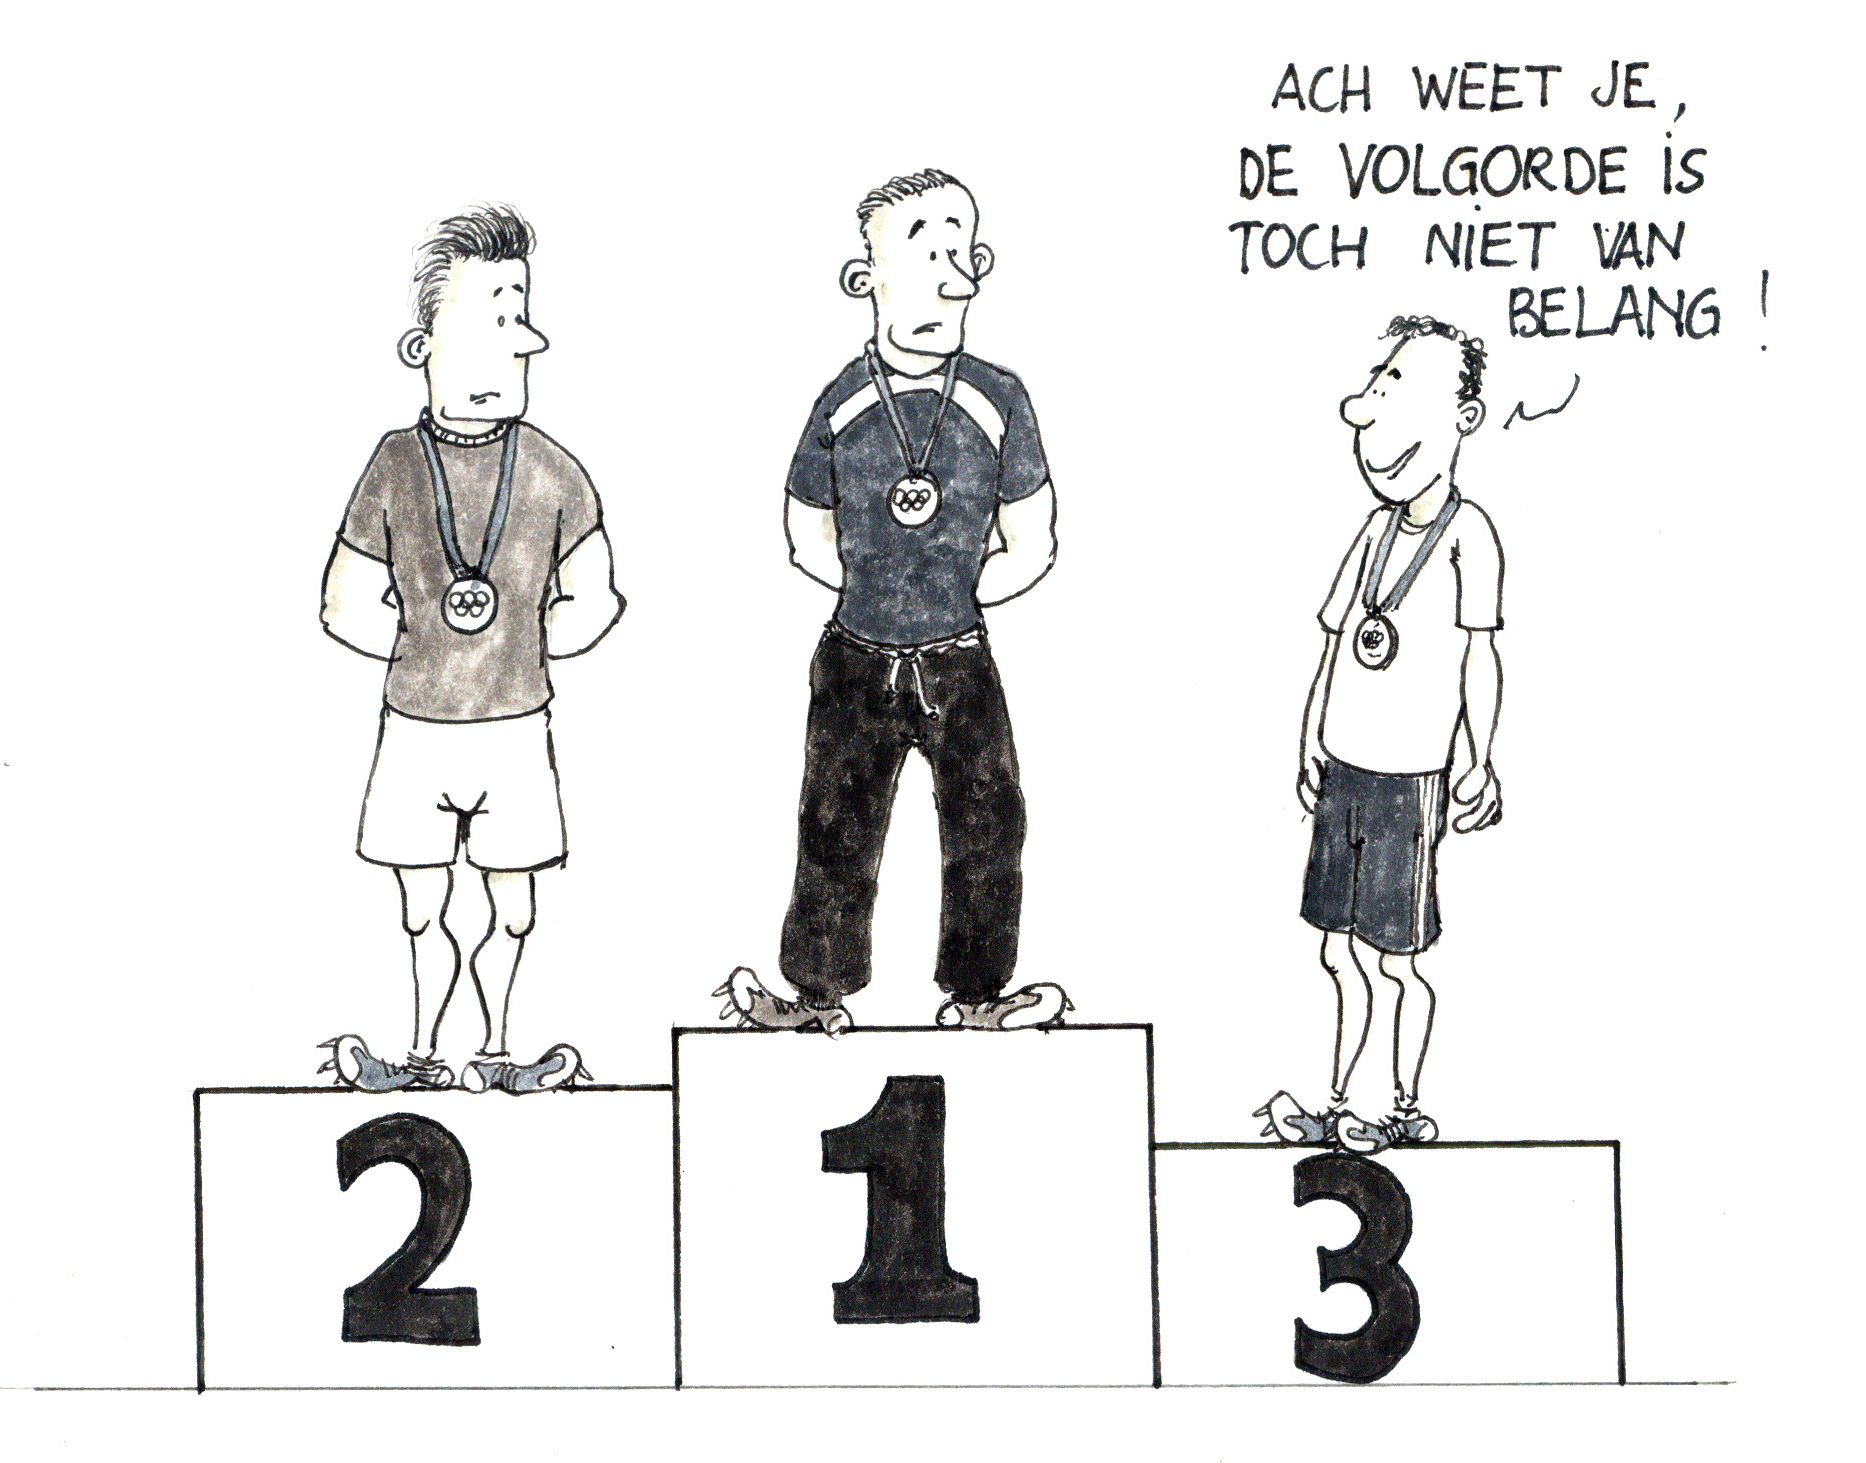
\includegraphics[width=\linewidth]{tekeningenKurt/volgordenietvanbelang.jpg}
\end{figure} 

\begin{werktekstoef}

\item {Wat tel je? Geef enkele voorbeelden.}

\emph{Je telt duo’s van leerlingen, bv.  Bob en Cheb, Ahmed samen met Dora ... We kunnen alle mogelijkheden hier met de voorletters opsommen: AB, AC, AD, ...}

\item{Over welk element gaat het in deze telling?}

\emph{Een leerling.}

\item{Hoeveel elementen zijn er ter beschikking?}

\emph{n=$5$}

\item{Hoeveel elementen moet je kiezen?}

\emph{p=$2$}

\item {Hebben de geselecteerde elementen een bepaalde rol? Geeft een andere volgorde een andere mogelijkheid? Verklaar.}

\emph{Neen, de geselecteerde leerlingen hebben geen bepaalde rol binnen het duo. Nee, een andere volgorde geeft nog steeds hetzelfde duo klasvertegenwoordigers: het duo Ahmed en Dora is hetzelfde als het duo Dora en Ahmed.}

\item {Kan je een element meerdere malen kiezen? Verklaar.}

\emph{Neen, je kan niet twee keer dezelfde leerling kiezen.  Dan zijn er geen twee klasvertegenwoordigers meer.}

\end{werktekstoef}

\eindewerktekst

\begin{multicols}{2} 

\section{Notaties bij combinatieleer}

Uit de vorige paragraaf blijkt dat verschillen in opgaven vaak draaien rond vragen over de volgorde van de elementen en of een element meerdere malen mag voorkomen. Afhankelijk hiervan spreken we van variaties, combinaties en herhalingsvariaties of -combinaties. Zo leidt methode 1 in de vorige werktekst tot een variatie en methode 2 tot een combinatie. 
 
\end{multicols}

\tussentitel{Schema: we kiezen $p$ uit $n$ elementen}

\begin{center}
\begin{tabular}{|c|c|c|}
\cline{2-3}
\multicolumn{1}{c|}{} & &\\
\multicolumn{1}{c|}{} & een andere volgorde van & een andere volgorde van\\
\multicolumn{1}{c|}{} & de elementen geeft GEEN & de elementen geeft WEL EEN\\
\multicolumn{1}{c|}{} & andere mogelijkheid & andere mogelijkheid\\
\multicolumn{1}{c|}{} & &\\
\hline
&&\\
een element kan NIET & aantal combinaties: & aantal variaties: \\
meerdere malen voorkomen & $C_n^p$ & $V_n^p$ \\
 & &  aantal permutaties:\\
 & & $P_n$ als $p=n$\\
&&\\
\hline
&&\\
een element kan WEL & aantal herhalingscombinaties: & aantal herhalingsvariaties: \\
meerdere malen voorkomen & $\overline{C}_n^p$ & $\overline{V}_n^p$ \\
 & & aantal herhalingspermutaties:   \\
 & & $\overline{P}_n^{p_1,p_2, \dots}$ met $p_1+p_2+\dots=n$  \\
&&\\
\hline
\end{tabular}
\end{center}

\vspace{1cm}

\begin{multicols}{2}
In handboeken brengt men deze groeperingsvormen vaak per soort aan. Het nadeel is dat oefeningen ook gegroepeerd zijn per soort en men niet voldoende geconfronteerd wordt met nadenken over het onderscheid tussen de groeperingsvormen. Wij kiezen er voor om onmiddellijk eenvoudige oefeningen door elkaar aan te bieden zodat leerlingen  deze `basis'opgaven vlot leren herkennen. Dit levert een nieuwe methode op, naast het werken met systematische methodes en met de som-, product- en complementregel. Deze nieuwe methode kunnen de leerlingen gebruiken om moeilijkere of samengestelde problemen op te lossen. We zetten dus vooral in op het aanleren van basistechnieken om de juiste groeperingsvorm te herkennen. 

De notaties en formules brengen we in twee stappen aan. Eerst introduceren we in een schema de namen en notaties van de groeperingsvormen zonder de formules. Vervolgens analyseren we typevoorbeelden zonder het aantal mogelijkheden te berekenen (paragraaf 4). De essentie bij deze aanvangsoefeningen is dat leerlingen het onderscheid tussen de verschillende types leren kennen en hun keuze correct kunnen verantwoorden. 

De formules om aantallen te berekenen, brengen we pas aan nadat leerlingen geoefend zijn in het bepalen van naam en notatie van de groeperingsvorm (paragraaf 5). 

\section{Typevoorbeelden}

In de volgende werktekst bieden we zes typevoorbeelden aan en oefenen de leerlingen de zes vragen in. Naargelang van de antwoorden op deze vragen, leren de leerlingen de verschillende typen van problemen onderscheiden. Ze denken na over het soort telprobleem en oefenen de notatie uit het schema in. 

In wiskundeluwe richtingen kun je je beperken tot vier typevoorbeelden. De herhalingspermutatie en de herhalingscombinatie kunnen hier wegvallen.

Een mogelijke keuze van typeproblemen geven we hieronder:

\begin{nummering}
\item een delegatie van leerlingen uit een  klas naar een overleg sturen (typeprobleem voor het tellen van combinaties);
\item een top drie van favoriete muzieknummers (typeprobleem voor het tellen van variaties);
\item de hele klas in een rij laten aanschuiven in het schoolrestaurant (typeprobleem voor het tellen van permutaties);
\item een cijferslot van een bankkluis instellen (typeprobleem voor het tellen van herhalingsvariaties);
\item alle balletjes uit een kookpot met tomatensoep verdelen over de borden van de kinderen (typeprobleem voor het tellen van herhalingscombinaties);
\item anagrammen maken van het woord ANANASSAP (typeprobleem voor het tellen van herhalingspermutaties).
\end{nummering}

De laatste twee opdrachten zijn geen verplichte leerstof voor wiskundeluwe studierichtingen. Toch zijn ze interessant vooral voor leerlingen die verder studeren en telproblemen op het menu krijgen. Stel de situatie goed voor om antwoorden te vinden op de vragen.

We geven hieronder een idee van de opbouw van de werktekst. We behandelen één typevoorbeeld volledig. Van de andere voorbeelden behandelen we enkel de vijfde vraag.

\end{multicols}

\beginwerktekst{Typevoorbeelden en combinatieleer}

Beantwoord bij de onderstaande opdrachten de zes vragen voor het analyseren van telproblemen. Omcirkel vervolgens de juiste formule.

\tussentitel{Een delegatie sturen}

Hoeveel mogelijkheden zijn er om een delegatie van 5 leerlingen uit een klas met 21 leerlingen naar een overleg met de directie te sturen?

\begin{werktekstoef}

\item {Wat tel je? Geef hierbij enkele voorbeelden.}

\emph{We tellen groepen van 5 leerlingen, bv. Ahmed, Bob, Cheb, Dora en Ems.}

\item{Over welk element gaat het in deze telling?}

\emph{Een leerling van de klas.}

\item{Hoeveel elementen zijn er ter beschikking?}

\emph{$n=21$}

\item{Hoeveel elementen moet je kiezen?}

\emph{$p=5$}

\item {Hebben de geselecteerde elementen een bepaalde rol? Geeft een andere volgorde een andere mogelijkheid?}

\emph{Neen, de geselecteerde leerlingen hebben geen bepaalde rol. Het zijn vertegenwoordigers. Neen, een andere volgorde van kiezen geeft geen andere delegatie.}

\item {Kun je een element meerdere keren kiezen? Verklaar.}

\emph{Neen, je kunt niet twee keer dezelfde leerling kiezen, want dan heb je te weinig delegatieleden.}

\end{werktekstoef}

De formule is \ $C_n^p$\ \ \ $V_n^p$\ \ \ $P_n$\ \ \ $\overline{C}_n^p$ \ \ \ $\overline{V}_n^p$ \ \ \ $\overline{P}_n^{p_1,p_2, \dots}$

\tussentitel{De top drie}

Hoeveel mogelijkheden zijn er om een top drie van favoriete songs op te stellen uit een lijst van 1000 songs? 

\begin{werktekstoef}
\setcounter{enumi}{4}
\item{Hebben de geselecteerde elementen een bepaalde rol? Geeft een andere volgorde een andere mogelijkheid?}

\emph{Ja, de eerste song is de meest favoriete song. Ja, als je de volgorde wijzigt geeft dat een andere top drie.}
 \end{werktekstoef}
 
\tussentitel{Het schoolrestaurant}

Op hoeveel manieren kan een klas van 20 leerlingen in een rij aanschuiven in het schoolrestaurant? 

\begin{werktekstoef}
\setcounter{enumi}{4}
\item{Hebben de geselecteerde elementen een bepaalde rol? Geeft een andere volgorde een andere mogelijkheid?}

\emph{Ja, de plaats van de leerling in de rij is belangrijk. Ja, als leerlingen in een andere volgorde staan, geeft dit een andere mogelijkheid. De leerling die eerst in de rij staat, moet minder lang aanschuiven en heeft misschien de grootste keuze uit het buffet.}
\end{werktekstoef}

\tussentitel{Het cijferslot}

Op hoeveel manieren kun je een cijferslot van 4 cijfers voor een fiets instellen?

\begin{werktekstoef}
\setcounter{enumi}{4}
\item{Hebben de geselecteerde elementen een bepaalde rol? Geeft een andere volgorde een andere mogelijkheid?}

\emph{Ja, bij een cijferslot hangt de plaats van de cijfers vast aan het radertje dat je kunt draaien. Het meest linkse cijfer heeft een andere rol dan het tweede cijfer. Ja, een andere volgorde geeft een andere code: $0473$ is een andere code dan $7304$.}
\end{werktekstoef}

\tussentitel{Soep met balletjes}

Op hoeveel manieren kan vader de 15 balletjes uit een kookpot met tomatensoep verdelen over de borden van vier kinderen?

\begin{werktekstoef}

\item {Wat tel je? Geef hierbij enkele voorbeelden.}

\emph{Je kiest $15$ keer een bord waarin je een balletje legt. De verdeling van balletjes over $4$ borden kan dus zijn: het eerste bord wordt $0$ keer gekozen en heeft dus $0$ balletjes, het tweede bord wordt $5$ keer gekozen, het derde bord $7$ keer en het vierde bord $3$ keer. Het rijtje $0, 5, 7, 3$ beschrijft de verdeling van de balletjes over de borden. We tellen deze verdelingen.}

\item{Over welk element gaat het in deze telling?}\\
\emph{Er wordt telkens een bord gekozen.}

\item{Hoeveel elementen zijn er ter beschikking?} \\
\emph{$n=4$}

\item{Hoeveel elementen moet je kiezen?}\\
\emph{$p=15$}

\item {Hebben de geselecteerde elementen een bepaalde rol? Geeft een andere volgorde een andere mogelijkheid?}\\
\emph{Neen, hoewel een bord bij een kind hoort, hangt aan het leggen van een balletje in een bepaald
bord geen rol. Neen, de volgorde waarin de vader een bord kiest, heeft geen effect op het aantal balletjes dat
uiteindelijk in elk bord ligt. Zo kan vader 5 opeenvolgende keren bord 2 kiezen en daarna 5 opeenvolgende keren bord 3. Hij kan ook 5 keer afwisselend een balletje in bord 2 en 3 leggen. Het resultaat is dan hetzelfde ondanks de andere volgorde waarin de borden gekozen werden.}

\item {Kun je een element meerdere keren kiezen? Verklaar.}\\
\emph{Ja, vader kan (en moet) sommige borden meerdere keren kiezen.}

\end{werktekstoef}

\tussentitel{Ananassap}

Hoeveel anagrammen kun je maken van het woord ANANASSAP? Beantwoord de zes typevragen voor het analyseren van telproblemen.

\begin{werktekstoef}
\setcounter{enumi}{4}
\item {Hebben de geselecteerde elementen een bepaalde rol? Geeft een andere volgorde een andere mogelijkheid?}

\emph{Ja, de plaats van een letter in een woord speelt een rol in de betekenis van het woord. Ja, een andere volgorde van de letters geeft een ander woord: KAM is een ander woord dan MAK.}

\item {Kun je een element meerdere keren kiezen? Verklaar.}

\emph{Dit woord heeft $9$ letters maar ze zijn niet allemaal verschillend: de A komt $4$ keer voor, de N en de S $2$ keer en de P $1$ keer. Sommige letters moet je dus meermaals kiezen om een zuiver anagram te krijgen. Deze  groeperingsvorm (van letters) noemt men een herhalingspermutatie met $p_i$ achtereenvolgens gelijk aan $4, 2, 2$ en $1$. Hierbij is de som van de $p_i$'s gelijk aan het aantal letters: $4+2+2+1=9$.}

\end{werktekstoef}
De bovenstaande voorbeelden noemen we typevoorbeelden. Als je het typevoorbeeld herkent, weet je of de groeperingen een combinatie, variatie, permutatie, herhalingsvariatie, herhalingscombinatie of herhalingspermutatie is. 

Onthoud de volgende woorden om naar typevoorbeelden te verwijzen: delegatie (combinatie), top drie (variatie), schoolrestaurant (permutatie), cijferslot (herhalingsvariatie) en als uitbreiding soepballetjes (herhalingscombinatie) en ananassap (herhalingspermutatie).

\eindewerktekst

\begin{multicols}{2}

\section{Berekeningen bij combinatieleer}
Nu de typeproblemen gekend zijn, is het tijd om te rekenen. We vullen het schema aan met formules en met de instructies om met de rekenmachine te rekenen. Schattingen van de inleidende werktekst kunnen dan gecontroleerd worden en de antwoorden op de typevoorbeelden geformuleerd.\\ 

In deze loep besteden we weinig aandacht aan het opstellen van de formules. Die vind je namelijk terug in bijna alle handboeken over dit thema. We willen hiermee niet in herhaling vallen. In de sterke richtingen moeten deze formules vlot gekend zijn. In wiskundeluwe richtingen kunnen de leerlingen zich beperken tot het  opvragen van deze combinatorische getallen met hun rekenmachine. In de tussenrichtingen kan er gedifferentieerd worden, naargelang van de mogelijkheden en de interesses van de leerlingen.
\end{multicols}

\tussentitel{Schema: aangevuld met formules en instructies voor het grafisch rekentoestel (GRM)}

\begin{center}
\begin{tabular}{|c|c|c|}
\cline{2-3}
\multicolumn{1}{c|}{} & &\\
\multicolumn{1}{c|}{} & een andere volgorde van & een andere volgorde van\\
\multicolumn{1}{c|}{} & de elementen geeft GEEN & de elementen geeft WEL EEN\\
\multicolumn{1}{c|}{} & andere mogelijkheid & andere mogelijkheid\\
\multicolumn{1}{c|}{} & &\\
\hline
&&\\
een element kan NIET & aantal combinaties: & aantal variaties: \\
meerdere malen voorkomen & $C_n^p=\frac{n!}{p!\cdot(n-p)!}$ \qquad GRM: $nCp$ & $V_n^p=\frac{n!}{(n-p)!}$  \qquad  GRM: $nPp$\\
 & &  aantal permutaties:\\
 & & $P_n=n$! \qquad GRM: $n!$\\
&&\\
\hline
&&\\
een element kan WEL & aantal herhalingscombinaties: & aantal herhalingsvariaties: \\
meerdere malen voorkomen & $\overline{C}_n^p$=$C_{n+p-1}^p$ & $\overline{V}_n^p$=$n^p$ \\
 & & aantal herhalingspermutaties:   \\
 & & $\overline{P}_n^{p_1,p_2, \dots} =\frac{n!}{p_1!p_2!\dots}$\\
&&\\
\hline
\end{tabular}
\end{center}

%\vspace{0.5cm}

\begin{multicols}{2}

In de laatste fase van het aanleren van deze basistelproblemen bieden we een werktekst met twintig oefeningen aan waarbij de leerlingen de juiste groeperingsvorm bepalen aan de hand van de zes vragen. Ze vergelijken het probleem met een typeprobleem, bepalen de notatie en formuleren een antwoord op de vraag naar het aantal.

We werkten bij de werktekst een zelfverbeterende quiz uit via de website socrative.com. De leerlingen lossen bij elke oefening een multiplechoicevraag op en krijgen meteen een korte verantwoording bij het juiste alternatief.  In figuur \ref{socrative} zie je een voorbeeld van zulke multiplechoicevraag. In de verantwoording krijgen de leerlingen bij het juiste alternatief het typevoorbeeld en het combinatorisch getal. 

Socrative laat toe een spelelement toe te voegen via de optie `Space Race'. Je kunt leerlingen individueel of in groepjes tegen elkaar laten racen. Als je de strijd projecteert, verhoogt de competitie tussen de leerlingen. In figuur \ref{spacerace} tonen de fietsen de verschillende groepjes. Bij elk correct antwoord gaat de fiets vooruit. De winnaars zijn zij die de meeste oefeningen juist oplossen. De snelheid waarmee de vragen opgelost worden, heeft minder belang.

In de werktekst hieronder behandelen we vijf oefeningen. Deze werktekst is bedoeld voor wiskundeluwe richtingen. Je zult merken dat herhalingscombinaties en -permutaties niet voorkomen. De volledige tekst met twintig oefeningen vind je op onze website.

\end{multicols}

\begin{figure}[H]
\centering
\includegraphics[width=\linewidth]{figurenAuteur/socrativevraag.PNG}
\caption{Multiplechoicevraag in Socrative}
\label{socrative}
\end{figure}

\begin{figure}[H]
\centering
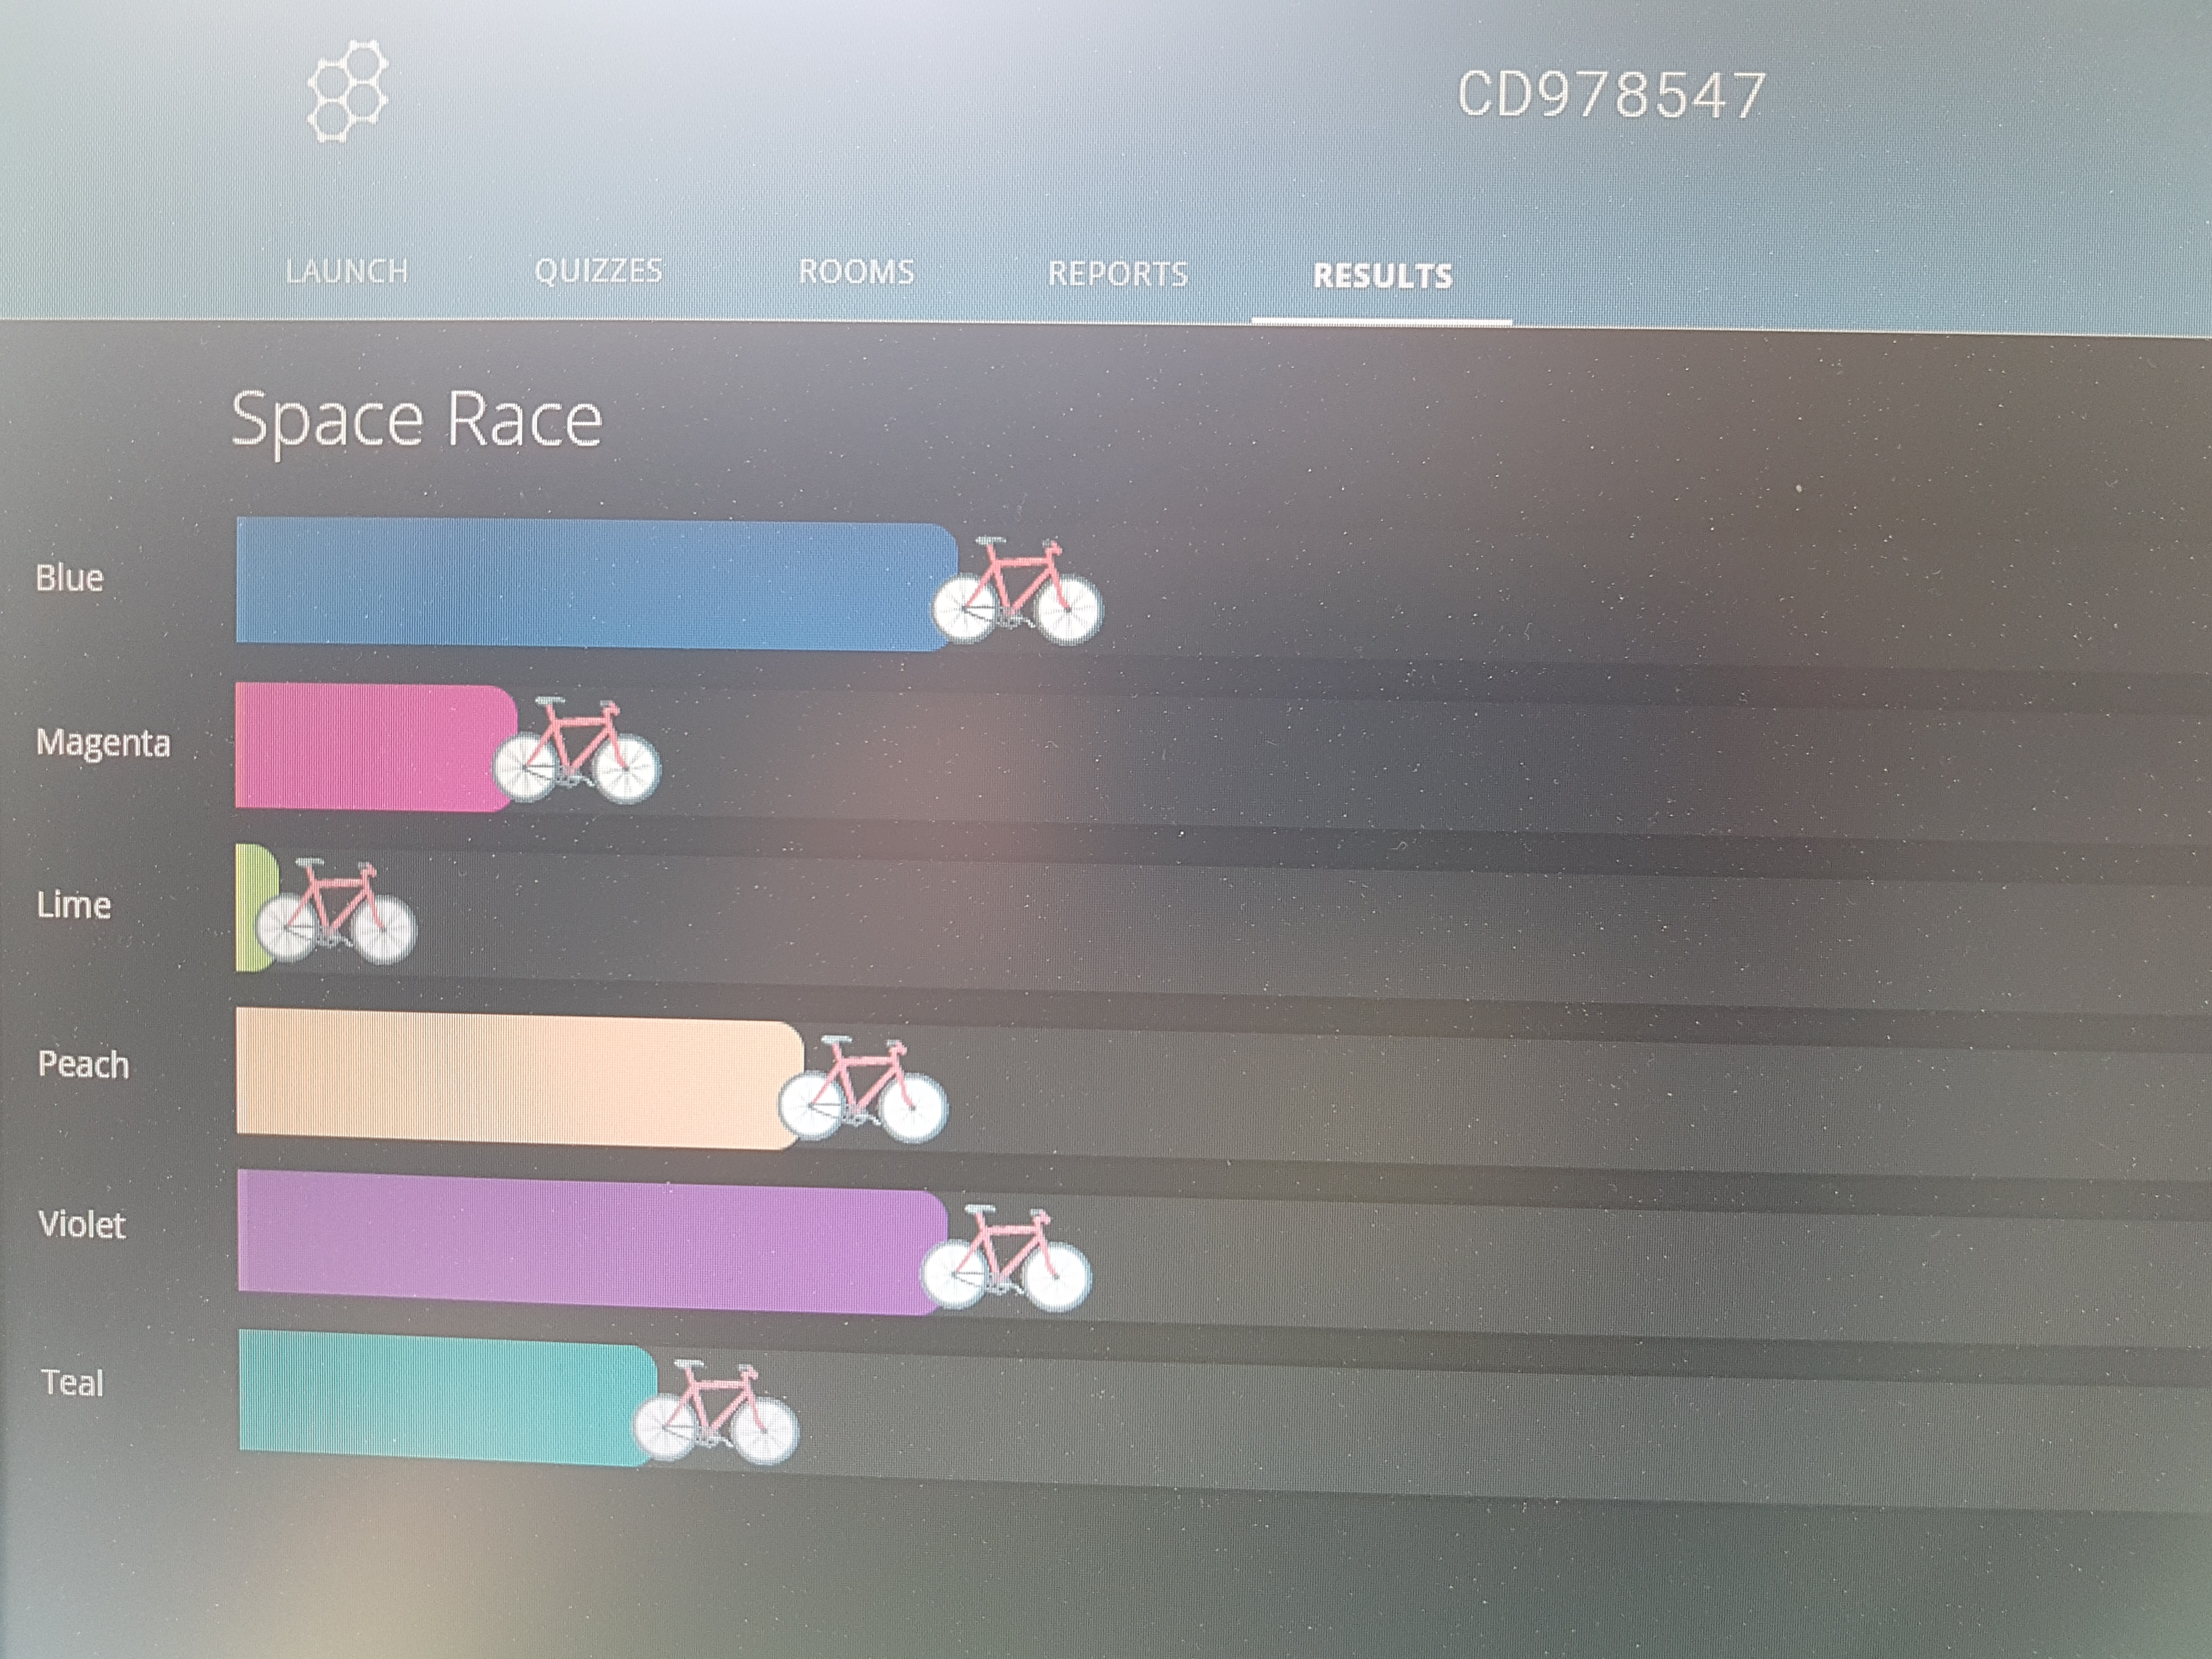
\includegraphics[width=0.70\linewidth]{figurenAuteur/spacerace.jpg}
\caption{Zes groepen in een Space Race}
\label{spacerace}
\end{figure}




\beginwerktekst{Telproblemen en notaties}

Door veel te oefenen krijg je inzicht in telproblemen. Hieronder volgen twintig basistelproblemen. Je gaat na of het om een variatie, permutatie, combinatie of herhalingsvariatie gaat en je duidt de formule aan waarmee je het aantal kunt bepalen. Je zet bij elk probleem het typevoorbeeld waarmee het overeenstemt. Gebruik hiervoor de volgende woorden: delegatie, top drie, schoolrestaurant of cijferslot. Je kunt je antwoorden controleren via Socrative. Open de app en gebruik CD978547 als 'roomnumber'. Als je merkt dat je een fout maakt, moet je de voorbeelden grondiger analyseren en de gestelde vragen nauwgezet beantwoorden. Zo kun je merken waar je fout redeneert. 

\begin{werktekstoef}

\item{Je hebt twee extra vrijkaarten voor een jazzfestival. Je wilt twee vrienden meenemen naar het festival door hen de vrijkaarten te geven. Hoeveel mogelijkheden zijn er om je twee kaarten weg te geven aan twee van je zes beste vrienden zodat ze met je mee kunnen gaan naar het festival?}\\

\emph{Ik tel duo’s van vrienden waar ik een kaart aan geef. De geselecteerde vrienden hebben geen specifieke rol. Het maakt niet uit of ik eerst een kaart aan Lieve geef en dan aan Tine of juist andersom. Het duo Lieve, Tine krijgt een vrijkaart. Ik kies niet tweemaal eenzelfde vriend. Je kunt deze hele redenering samenballen in het woord 'delegatie'. Er zijn 10 delegaties mogelijk.}

\item {Bij het spelletjes Mastermind plaats je vier pinnetjes te kiezen uit zes kleuren (rood, groen, blauw, geel, bruin en oranje) op een bord in een bepaalde volgorde. De pinnetjes hoeven niet noodzakelijk verschillend van kleur te zijn.  Bereken het aantal mogelijkheden om vier pinnetjes te plaatsen.}\\
\emph{Een voorbeeld is (rood, rood, groen, geel). Je kiest het element kleur. Elke plaats op het bord heeft zijn rol. Dus in het voorbeeld staat op de meest linkse plek een rood pinnetje, een rood daarnaast enz… In de opgave staat dat de pinnetjes op een bepaalde volgorde gezet worden. De volgorde rood, rood, groen, geel is niet hetzelfde als groen, rood, geel, rood. Je mag kleuren herhalen. Het typevoorbeeld is het `cijferslot'. Je kunt op $1296$ manieren vier pinnetjes uit zes kleuren kiezen en ze in een bepaalde volgorde op het bord plaatsen.}

\item {In het kader van hun studiekeuze moeten de leerlingen van het zesde jaar een persoon die een job uitoefent die hen interesseert, een dag volgen. De vijftien leerlingen van een klas kunnen kiezen uit vijftien verschillende personen. Op hoeveel verschillende manieren kan dit als elke leerling een andere persoon moet kiezen.}\\
\emph{Ik tel lijsten met personen die gevolgd zullen worden door leerlingen. De $15$ beroepen (of personen die dit beroep uitoefenen) vul ik in op een klaslijst. De eerste persoon hoort dus bij de leerling die eerst op de klaslijst staat. De volgorde van de beroepen is van belang. Het typeprobleem is het `schoolrestaurant'. De vijftien leerlingen van een klas kunnen op $1,31 \cdot 10^{12}$ manieren een persoon kiezen die ze een dag zullen volgen.}

\item {Op het onderstaande \emph{mini-Lotto}-formulier moeten drie van de vijf vakjes worden aangekruist. Hoeveel mogelijkheden zijn er om dit te doen?}

\begin{figure}[H]
\centering
\includegraphics[width=0.3\linewidth]{figurenAuteur/minilotto.png}
\end{figure}

\emph{Het element is een vakje of een getal. De volgorde van de geselecteerde getallen heeft geen belang. Of je eerst het vakje $1$, dan $3$ en als laatste $4$ aankruist of eerst $3$, dan $1$ en dan $4$, het resultaat blijft hetzelfde. Het typevoorbeeld is dat van de `delegatie'. Antwoord: er zijn $10$ manieren om $3$ van de $5$ vakjes aan te kruisen op het `mini-Lotto'-formulier.}

\item {Een zaal heeft vijf deuren. Op hoeveel manieren kan iemand de zaal binnenkomen en de zaal door een andere deur verlaten?}

\emph{Elke geselecteerde element (deur) heeft een rol, de deur hoort bij het binnen- of buitengaan van de zaal. Zo kun je stellen dat de eerste deur van het duo bij het binnenkomen hoort en de tweede bij het buitengaan. Vermits je door een andere deur de zaal moet verlaten dan dat je binnenkomt, kun je een element niet opnieuw kiezen. Het typevoorbeeld is hier de 'top drie'. Het gaat om het aantal variaties van $2$ elementen uit $5$. Dit getal is gelijk aan $20$.}

%\item {In een multiplechoicetest worden vier vragen gesteld, met op elke vraag 3 mogelijke antwoorden. Op hoeveel manieren kan men een toetsformulier invullen als voor elke vraag juist één antwoord moet gegeven worden?}\\
%\emph{Ik tel setjes van 4 mogelijke antwoorden op vragen. Stel dat de mogelijke antwoorden A, B en C zijn. Een voorbeeld is AABB. De elementen (antwoordalternatieven) hebben een rol. De eerste letter hoort bij de eerste vraag, de tweede bij de tweede vraag enz. In het voorbeeld is het antwoord op de vragen: 1A, 2A, 3B en 4B. Als je dit rijtje wijzigt in ABBA dan is het antwoord op twee vragen gewijzigd, nl. 1A, 2B, 3B, 4A.}

\end{werktekstoef}

\eindewerktekst

\begin{multicols}{2}

\tussentitel{Exit ticket en Kahoot}

De werktekst met de 20 oefeningen neemt maximaal twee uur in beslag. Niet alle groepen slagen er in om alle oefeningen op te lossen. Op het einde van het tweede lesuur vullen de leerlingen individueel een `exit ticket' in met één of twee heel korte vragen. Dit heeft de bedoeling om snel te testen of de lesdoelen bereikt zijn. 

Na de les komt de verbetersleutel online. De leerlingen kunnen alles nog eens grondig doornemen ter voorbereiding van de volgende les. Dan volgt een tweede quiz, deze keer gemaakt op kahoot.com. In de multiple choice quiz komen dezelfde 20 opgaven aan bod. Hij dient als herhalings- en evaluatietool. De leerlingen moeten ditmaal op tempo multiple choice vragen oplossen.
Per vraag toont kahoot telkens het juiste antwoord en het aantal leerlingen of duo's dat juist antwoordde. Daarnaast krijg je telkens de totaalstand. Je hebt snel een overzicht het aantal correcte antwoorden. Via een onderwijsleergesprek kan de verantwoording per oefening nog eens aan bod komen. Hier blijken de leerlingen niet altijd even sterk in. Zeker is dat zij die hun antwoord goed kunnen uitleggen, verderop nauwelijks nog fouten maken. 

De kahootquiz vind je via 
\url{https://create.kahoot.it/share/telproblemen/88f30241-ccf0-4ee3-b3e0-bfcdad860fd2}

\section {Samengestelde problemen}

Telproblemen komen in onze leefwereld vaak niet in zuivere vorm voor: ze zijn meestal niet op te lossen met één enkel basistype. Sommige tellingen kunnen zelfs helemaal niet tot een van de basistypen herleid worden. Het vraagt heel wat behendigheid om bepaalde telproblemen in deelproblemen op te splitsen die aanleiding geven tot zuivere combinaties, variaties of permutaties, al of niet met herhalingen.

Voor het bundelen van de resultaten van deelproblemen bestaat er wel een vuistregel: gebruik een som als de deelproblemen aan elkaar gekoppeld zijn met het voegwoord \emph{of}, gebruik een product als ze verbonden worden met het voegwoord \emph{en}, gebruik een verschil wanneer de opgave \emph{niet}, \emph{behalve} of \emph{zonder} bevat.

\tussentitel {Een klassikaal voorbeeld}

Het opsplitsen in deelproblemen moet voldoende in de klas ingeoefend worden vooraleer de leerlingen in staat zijn om dit zelf te doen. Dit begeleid inoefenen kan gedaan worden via een klasgesprek maar het kan ook met werkteksten. Hieronder werken we een eerste oefening uit waarin het totale aantal autokentekens berekend wordt dat volgens de Europese regels kan gegenereerd worden.

\end{multicols}


\beginwerktekst{Autokentekens}

In het jaar 2010 schakelde België over op Europese autokentekens. In ons land hebben de Europese nummerplaten robijnrode letters en cijfers op een witte achtergrond met  een rode rand. Er rijden nog steeds een aantal oude autokentekens rond maar momenteel zijn de meeste kentekens van de vorm 1-ABC-123.

\begin{center}
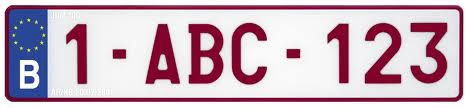
\includegraphics[width=0.4\linewidth]{figurenAuteur/Autokenteken.jpg}
\end{center}

De wet legt een beperking op aan het lettergedeelte. De letters I, O en Q worden niet gebruikt omdat ze te erg op de cijfers 1 en 0 gelijken. Verder zijn er 100 drieletterwoorden verboden omdat ze als scheldwoord kunnen opgevat worden (AAP, ZAK, ...), omdat ze een politieke betekenis hebben (CDH, CDV, ...) of omdat ze seksueel getint zijn (LUL, GAY, ...). 

\begin{werktekstoef}

\item{Hoeveel kentekens zijn er als je geen rekening moet houden met de verboden woorden maar wel met de verboden letters? Het cijfer voor de drie letters moet altijd 1 zijn.}

\emph{Het lettergedeelte bestaat uit $3$ letters die gekozen worden uit $23$ letters zoals bij het model van het cijferslot: $\overline{V}^3_{23}=23^3$. Het cijfergedeelte bestaat uit $3$ cijfers die gekozen worden uit $10$ cijfers zoals bij een cijferslot: $\overline{V}^3_{10}=10^3$. Aangezien er \emph{en} een lettergedeelte \emph{en} een cijfergedeelte nodig is, nemen we een product van deze twee getallen: $\overline{V}^3_{23} \cdot \overline{V}^3_{10}=23^3 \cdot 10^3= 12 167 000$.}

\item{Hoeveel bezwaarlijke autokentekens zijn er die beledigend, politiek of seksueel getint zijn?}

\emph{Er zijn $100$ lettergedeeltes verboden. Een nummerplaat bestaat uit een lettergedeelte \emph{en} een cijfergedeelte. Daarom maken we opnieuw een product: $100 \cdot \overline{V}^3_{10}=100 000$.}

\item{Hoeveel toegelaten kentekens zijn er die beginnen met het cijfer 1?}

\emph{De toegelaten kentekens zijn alle kentekens met uitzondering van de verboden kentekens. We nemen dus een verschil: $\overline{V}^3_{23} \cdot \overline{V}^3_{10}-100 \cdot \overline{V}^3_{10}=12 067 000.$}

\end{werktekstoef}

Dit aantal komt ongeveer overeen met het aantal inwoners van België. Indien het nodig mocht zijn, kan het eerste kencijfer van het kenteken later nog vervangen worden door een ander cijfer. Eventueel kunnen ook de letter- en cijferblokjes nog omgewisseld worden. Op deze manier hoopt men in de Europese Unie over genoeg kentekens te beschikken om enkele honderden jaren verder te kunnen.


\eindewerktekst

\begin{multicols}{2} 
\tussentitel{Kneepjes en standaardproblemen}

Bij het opsplitsen in deelproblemen helpt het om over een werkkoffer met standaardtechnieken te beschikken, waarvan je het antwoord kent zonder verdere analyse te moeten maken. Hieronder openen we onze werkkoffer en tonen we het nuttigste alaam.

Als je wilt tellen hoeveel \emph{deelverzamelingen} een verzameling met $n$ elementen heeft, geef je elk element twee kaartjes, eentje met ‘ja’ en eentje met ‘neen’. ‘Ja’ betekent ‘ik wil bij de deelverzameling behoren’ en ‘neen’ betekent ‘ik wil niet bij de deelverzameling horen’. Door alle elementen van de gegeven verzameling een deelnemingskaartje te laten opsteken, ligt de deelverzameling vast. Alle elementen die ‘Ja’ opsteken behoren immers tot de deelverzameling. Het aantal deelverzamelingen van een verzameling met $n$ elementen is bijgevolg gelijk aan het aantal kaartopstekingen: $\overline{V}_2^n=2^n$. Het kneepje dat hier gebruikt wordt, is een andere voorstellingswijze te kiezen voor de elementen die geteld worden.

Een ander standaardprobleem gaat over het aantal \emph{kortste wegen} in een rechthoekig stratenplan van $n$ blokjes op $m$ om van linksboven naar rechtsonder te gaan. Een korstste weg kan omschreven worden door $m$ stapjes in zuidelijke (Z) richting te zetten en $n$ in oostelijke richting (O) en dit in een willekeurige volgorde. Een kortste pad komt met andere woorden overeen met een woord dat bestaat uit $m+n$ lettertekens waarvan $m$ Z'en en $n$ O's. Het aantal kortste paden is bijgevolg gelijk aan: $\overline{P}_{m+n}^{n,m}=C_{m+n}^m=C_{m+n}^n$.

Op hoeveel manieren kun je $n$ personen rond een ronde tafel laten plaatsnemen? Dit is ook een van de gekende standaardproblemen. Het begrip \emph{ronde tafel} hoef je hier niet letterlijk te nemen. Het gaat over een tafel waarbij elke positie evenwaardig is. Het enige wat iets uitmaakt, is wie er aan je linkerzijde zit en wie er aan je rechterzijde zit. Om de telling eenvoudig te maken, kies je een tafelverantwoordelijke die, vooraleer hij plaats neemt, zijn rechterhand uitsteekt. De $n-1$ andere gasten gaan in een rij staan aan de rechterkant van de tafelverantwoordelijke. Dit kan op $P_{n-1}=(n-1)!$ manieren. Eens de rij gevormd is, kan de kring gesloten worden en is de tafelschikking vastgelegd. Er zijn dus $P_{n-1}=(n-1)!$ verschillende tafelschikkingen mogelijk. We komen hier nog op terug bij het hoofdstuk over de kleuringen.

Schikkingen waarbij bepaalde elementen naast of achter elkaar gezet worden, komen ook wel eens voor. Denk aan echtparen die bij elkaar blijven bij een bepaalde schikking, sokkenparen die niet gescheiden mogen worden ... Voor deze tellingen gebruik je de truc van het ducttapen. Kleef het echtpaar of het sokkenpaar met een ducttape samen tot één object en tel daarna het aantal schikkingen. Tot slot verwijder je de ducttape. 

\end{multicols}

\begin{figure}[H]
\centering
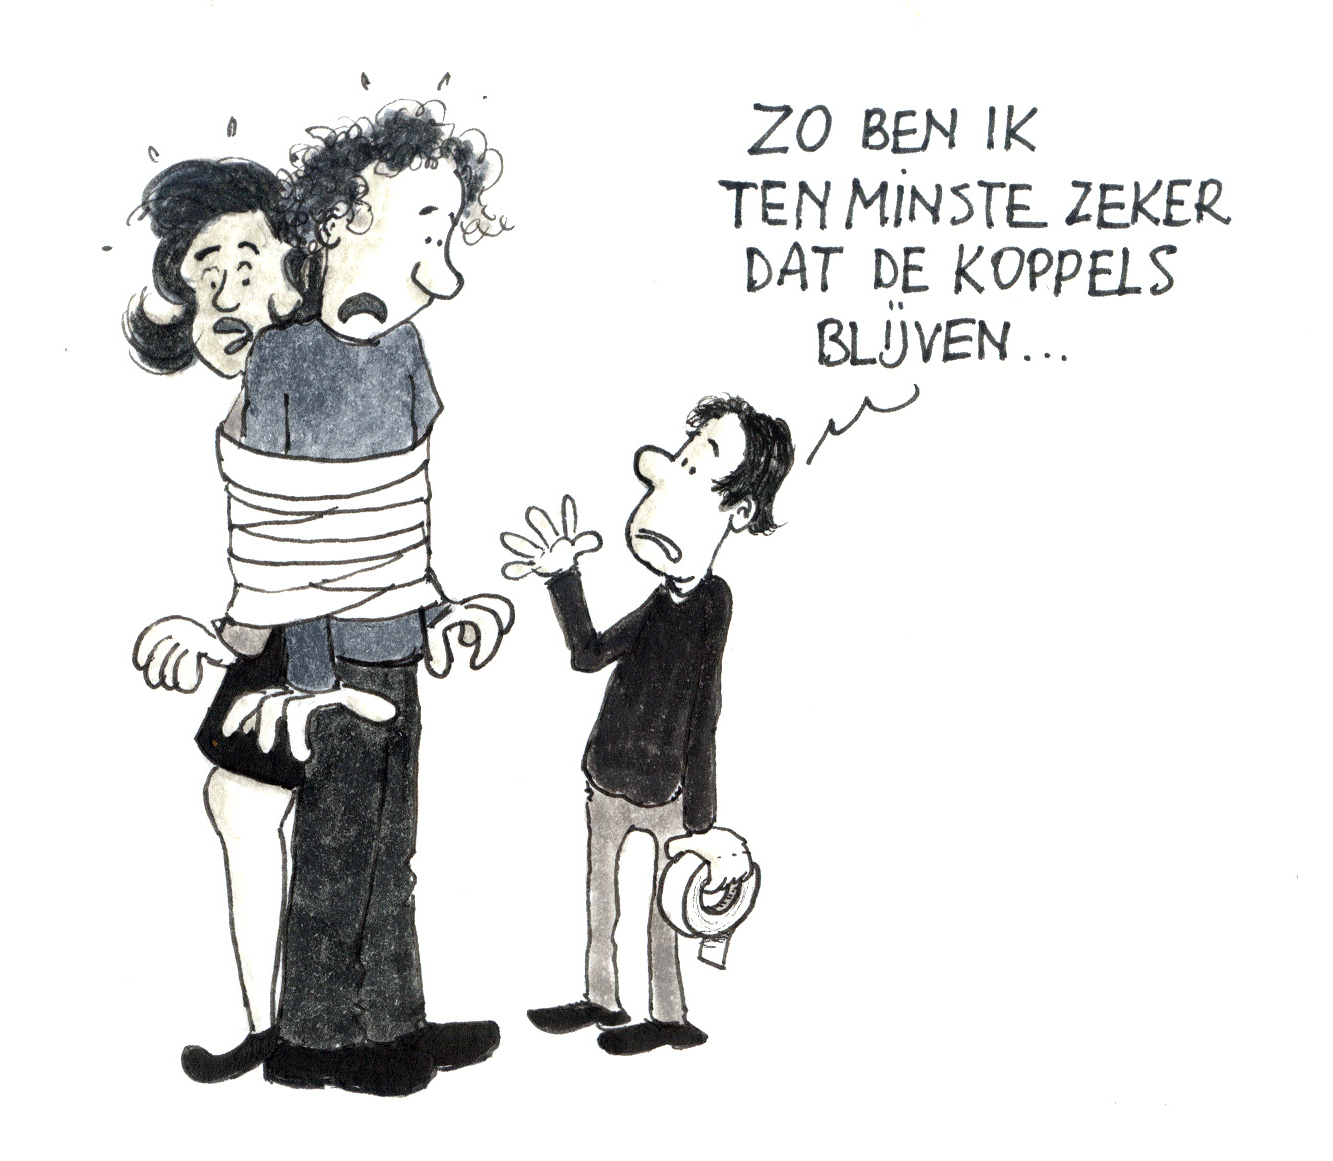
\includegraphics[width=0.65\linewidth]{tekeningenKurt/ducttape.jpg}
\end{figure} 

\begin{multicols}{2} 

Als er binnen de ducttape twee onderscheidbare objecten zitten (bijvoorbeeld een man en een vrouw) dan moet je het aantal schikkingen met twee vermenigvuldigen. Als de objecten niet onderscheidbaar zijn (zoals bij sokken) hoef je dit niet te doen.

\tussentitel {Een tweede klassikale voorbeeld}

We maken vervolgens een oefening op samengestelde telproblemen waarbij een van de standaardproblemen kan worden ingezet.

\end{multicols}

\beginwerktekst{Kortste wegen van huis naar school}

Hieronder zie je een rechthoekig stratenplan. Linksboven zie je de woonplaats (W) van Astrid  en rechtsonder zie je haar school (S). Op weg van huis naar school moet ze langs een flessenhals passeren. Er zijn vaak opstroppingen bij de post (P) en ook bij het gemeentehuis (G).

\begin{center}
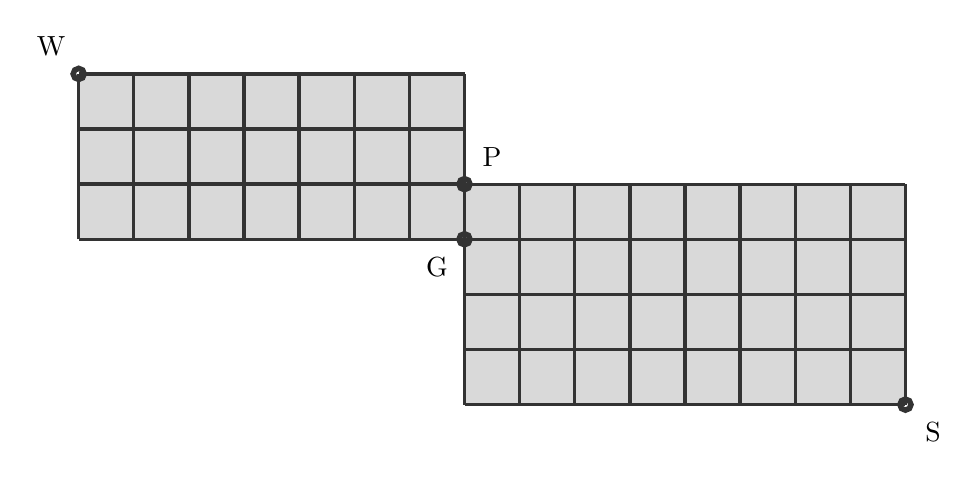
\begin{tikzpicture}[scale=0.7]
        \fill [color=gray!30] (0,3) -- (0,6) -- (7,6) -- (7,3);
        \fill [color=gray!30] (7,4) -- (15,4) -- (15,0) -- (7,0);
        \draw [very thick,black!80] (0,3) grid (7,6);
        \draw [very thick,black!80] (7,4) grid (15,0);
        \node at (-0.5,+6.5) {W};
        \draw[line width=2pt,color=black!80] (0,6) circle[radius=0.1];
        \node at (7.5,4.5) {P};
        \draw[line width=2pt,color=black!80] (7,4) circle[radius=0.1];
        \node at (6.5,+2.5) {G};
        \draw[line width=2pt,color=black!80] (7,3) circle[radius=0.1];
        \node at (15.5,-0.5) {S};
        \draw[line width=2pt,color=black!80] (15,0) circle[radius=0.1];
\end{tikzpicture}
\end{center}

Astrid kan op verschillende manieren van haar woning naar school fietsen zonder een omweg te doen. De enige voorwaarde om een kortste weg naar school te nemen is dat ze alleen in zuidelijke en in oostelijke richting rijdt.

\begin{werktekstoef}

\item{Op hoeveel manieren kan Astrid van haar woning naar school fietsen via de post?}

\emph{Om dit traject af te leggen moet ze een kortste pad van W naar P kiezen \emph{en} een kortste pad van P naar S. We passen hier de productregel toe. Het aantal kortste paden is: $C_9^2 \cdot C_{12}^4=36 \cdot 495= 17820$.}

\item{Hoeveel kortste trajecten zijn er via het gemeentehuis?}

\emph{Op eenzelfde manier berekenen we: $C_{10}^3 \cdot C_{11}^3=120 \cdot 165= 19800$.}

\item{Op hoeveel manieren kan Astrid van haar woning naar school fietsen zonder omwegen te maken?}

\emph{Astrid kan via de post naar school of via het gemeentehuis. Het voegwoord \emph{of} duidt op een optelling, althans indien het een exclusieve \emph{of} is. Echter, de \emph{of} is hier niet exclusief. Er zijn paden die langs het gemeentehuis én de post gaan. En deze wegen zijn  dubbel geteld. Die moet je dus nog van de som aftrekken. Het juiste antwoord is: $C_9^2 \cdot C_{12}^4+C_{10}^3 \cdot C_{11}^3-C_9^2 \cdot C_{11}^3=17820+19800-5940=31680$. }

\end{werktekstoef}

Een andere manier om dit antwoord uit te tellen, verloopt zonder veel voorkennis. Noteer bij elk kruispunt op hoeveel manieren je het kunt bereiken zonder omwegen te doen. Je begint bij het kruispunt 'W' linksboven en eindigt rechtsonder. Bij elke kruispunt dat niet op de rand gelegen is, schrijf je de som van het getal erboven en het getal links. Zo krijg je een schema dat verwant is met de driehoek van Pascal. Je merkt zelf wel dat het veel geduld vraagt om deze getalletjes verder uit te rekenen tot bij S.

\begin{center}
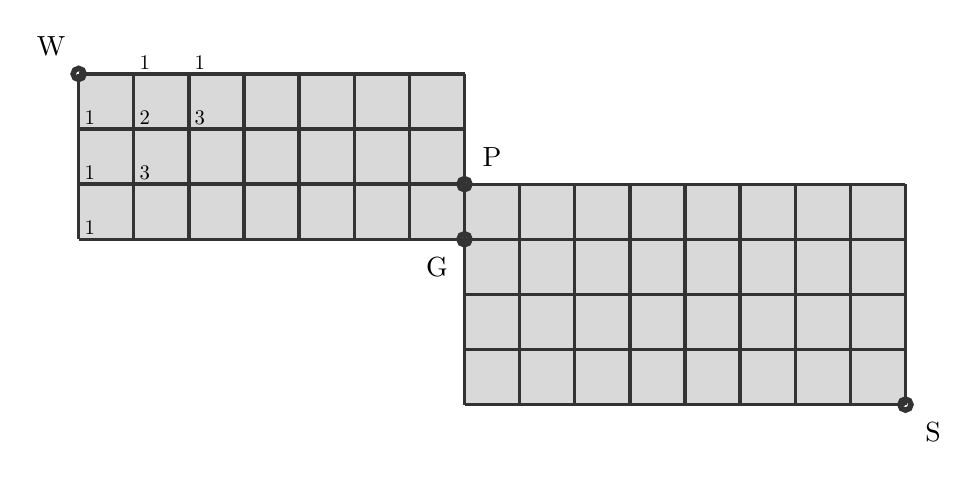
\begin{tikzpicture}[scale=0.7]
        \fill [color=gray!30] (0,3) -- (0,6) -- (7,6) -- (7,3);
        \fill [color=gray!30] (7,4) -- (15,4) -- (15,0) -- (7,0);
        \draw [very thick,black!80] (0,3) grid (7,6);
        \draw [very thick,black!80] (7,4) grid (15,0);
        \node at (-0.5,+6.5) {W};
        \draw[line width=2pt,color=black!80] (0,6) circle[radius=0.1];
        \node at (7.5,4.5) {P};
        \draw[line width=2pt,color=black!80] (7,4) circle[radius=0.1];
        \node at (6.5,+2.5) {G};
        \draw[line width=2pt,color=black!80] (7,3) circle[radius=0.1];
        \node at (15.5,-0.5) {S};
        \draw[line width=2pt,color=black!80] (15,0) circle[radius=0.1];
        \node [scale=0.75] at (1.2,6.2) {1};
        \node [scale=0.75] at (0.2,5.2) {1};
        \node [scale=0.75] at (1.2,5.2) {2};
        \node [scale=0.75] at (0.2,4.2) {1};
        \node [scale=0.75] at (1.2,4.2) {3};
        \node [scale=0.75] at (2.2,6.2) {1};
        \node [scale=0.75] at (2.2,5.2) {3};
        \node [scale=0.75] at (0.2,3.2) {1};
            
\end{tikzpicture}
\end{center}
\eindewerktekst

\begin{multicols}{2}
\tussentitel {Zelf een structuur bedenken voor de oplossing}

 Hoewel het zeer interessant kan zijn om leerlingen zelf een structuur te laten aanbrengen in de oplossing van een telprobleem, verwachten we deze vaardigheid eerder van leerlingen in een sterke wiskunderichting. Het vraagt heel wat inzicht. In de werktekst hieronder werden enkele samengestelde telproblemen bijeengebracht. Het is belangrijker de structuur te kunnen leggen in het antwoord dan de combinatorische getallen uit te kunnen rekenen.
 
\end{multicols}

\beginwerktekst{Drie samengestelde telproblemen}

\begin{werktekstoef}

\item{Een voetbaloutfit bestaat uit een petje, een sjaal, een truitje, een voetbalshort en twee kousen (linker- en rechterkous uiteraard van dezelfde kleur). Het voetbalteam van de school gebruikt de kleuren zwart, wit en rood. Hoeveel voetbaloutfits zijn er mogelijk waarbij alle kleuren voorkomen? Leg stapsgewijze uit hoe je dit aantal berekent.}

\emph{Een eerste soort kleuring is van het type RRZZW. Eén kleur komt één keer voor en twee kleuren komen twee keer voor. Er zijn drie mogelijkheden om de ene afzonderlijke kleur te kiezen. Stel dat deze kleur W is. Om de hele outfit in kleur te zetten, moet er dan een anagram gemaakt worden van de letters WRRZZ. Het totale aantal manieren om  kleuring van deze soort te maken is: $3 \cdot \overline{P}_5^{2, 2, 1}=90$. In klassen waarin de herhalingspermutatie niet gezien werd, kan die vervangen worden door een product van twee combinaties: $3 \cdot C_5^2 \cdot C_3^2$.
\\ \\
Een tweede soort kleuring is eentje van het type RRRWZ. Er komen twee enkele kleuren voor en één drietal. Er zijn drie mogelijkheden voor de keuze van de kleur van het drietal. Stel dat de kleur van het drietal W is. Dan kan de hele outfit gekleurd worden door een anagram te maken van WWWRZ. Het totaal aantal mogelijkheden voor deze kleuring is bijgevolg $3 \cdot \overline{P}_5^{3, 1, 1}=60$. Een redenering met combinaties geeft hetzelfde resultaat: $3 \cdot C_5^3 \cdot C_2^1$.\\ \\
Een kleuring met drie verschillende kleuren is \emph{ofwel} van het eerste type \emph{ofwel} van het tweede type. Er zijn geen andere mogelijkheden. We gebruiken dus de somregel:  $3 \cdot \overline{P}_5^{2, 2, 1}+3 \cdot \overline{P}_5^{3, 1, 1}=90+60=150$}.

\item{Een dodecaëderdobbelsteen heeft 12 zijvlakken met in de meeste uitvoeringen een getal van 1 tot 12 op de zijvlakken. Voor deze oefening mag je je deze dobbelstenen voorstellen met ogen. Deze voorstellingswijze is eenvoudiger. Bereken op hoeveel manieren er met vier dodecaëderdobbelstenen van een verschillende kleur 17 (ogen) kan gegooid worden.}

\begin{center}
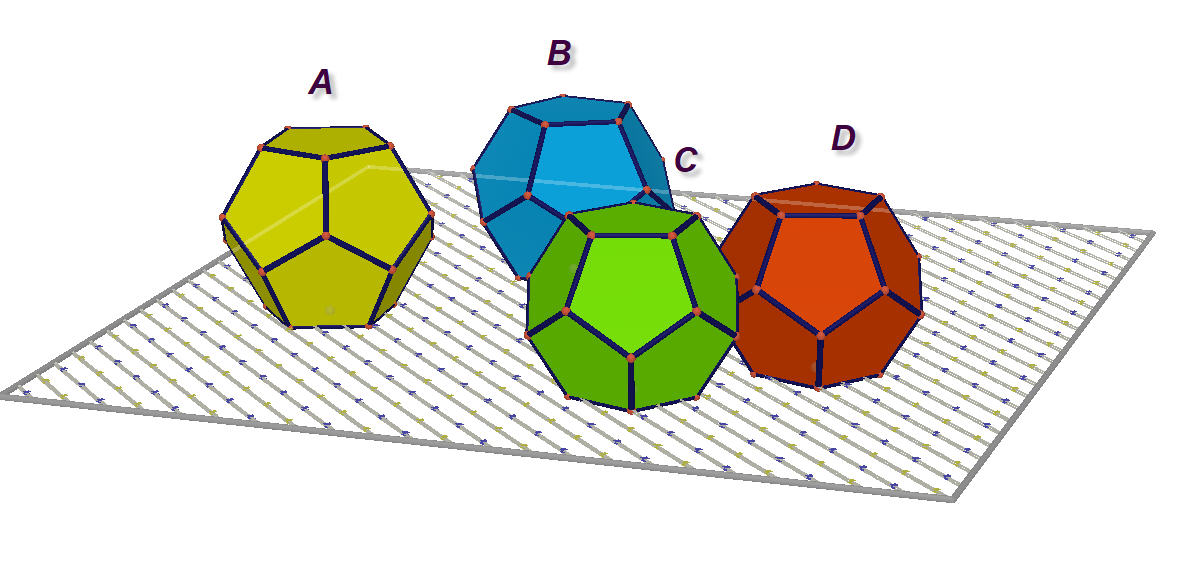
\includegraphics[width=0.8\linewidth]{figurenAuteur/dobbelstenen.jpg}
\end{center}

\emph{Het verdelen van $17$ ogen over de bovenvlakken van $4$ verschillende  dobbelstenen (A, B, C en D) lijkt op het verdelen van $17$ soepballetjes over vier soepborden. Er is echter een klein verschil: in een soepbord kunnen nul balletjes liggen maar op het bovenvlak van een dobbelsteen kunnen niet nul ogen staan. Daarom kleven we op elk bovenvlak al één oog. Er moeten dan nog maar $13$ ogen verdeeld worden over $4$ dobbelstenen. \\ \\ Deze $13$ ogen zijn identiek. Ze mogen dus verdeeld worden als soepballetjes over verschillende borden. We berekenen het aantal mogelijkheden met herhalingscombinaties: $\overline{C}_4^{13}=C_{16}^{13}=C_{16}^3=560$. \\ \\ De $13$ ogen mogen niet als volgt op de dobbelstenen komen: $13-0-0-0$ want dan zou de eerste dobbelsteen een bovenvlak hebben met $14$ ogen. Deze overtalligheid kan zich op $4$ manieren voordoen. Een verdeling van $12-0-1-0$ levert ook een dobbelsteen op die teveel ogen op het bovenvlak heeft. Deze onmogelijke situatie kan zich op $12$ manieren voordoen. Het totale aantal manieren om $17$ te gooien is dus $\overline{C}_4^{13}-4-12=560-16=544$. }

\item{KOOS U DE GARAGE DUS OOK is een palindromische zin. De letters van deze zin zijn spiegelsymmetrisch geschikt ten opzichte van de middelste letter, de R, maar de spaties hoeven dat bij een palindromische zin niet te zijn. Als ook de spaties symmetrisch zouden zijn, spreken we van een volmaakte palindroom. Volmaakte palindromen zijn veel zeldzamer dan gewone palindromische zinnen. Een voorbeeld hiervan is de geromantiseerde uitspraak die  Napoleon deed nadat hij naar Elba was verbannen: ABLE WAS I ERE I SAW ELBA. 

Hoeveel palindromische anagrammen zijn er van KOOS U DE GARAGE DUS OOK? De anagrammen hoeven geen betekenis te hebben. Ze moeten wel uit zes woorden bestaan. Leg grondig de structuur van je berekeningen uit.}

\emph{Als je geen rekening houdt met de spaties, dan vind je een palindromisch anagram van KOOSUDEGARAGEDUSOOK door een anagram te maken van het woord KOOSUDEGA. Dit anagram vul je aan met de letter R en vervolgens met het gespiegelde anagram. Het aantal anagrammen dat op deze manier gemaakt kan worden, is $\overline{P}_9^2=181 440$. \\ \\ Als je een palindromische anagram van KOOSUDEGARAGEDUSOOK in zes woorden wilt hakken, zijn er 18 posities mogelijk voor de spaties. Hier moeten er 5 van gekozen worden. Er mag geen herhaling optreden bij de posities. Wanneer een positie voor een spatie gekozen is, valt ze weg. De volgorde van het kiezen van de positie voor de spaties is ook niet van belang. Het aantal manieren om de spaties te zetten, wordt dus berekend met combinaties: $C_{18}^5=8 568$. \\ \\ Om een correct palindromisch anagram van zes woorden te maken, moeten we eerst een anagram zonder spaties maken en daarna de spaties toevoegen. We horen het voegwoord \emph{en} en maken daarom gebruik van de productregel: $\overline{P}_9^2 \cdot C_{18}^5= 181 440 \cdot 8 568= 1 554 577 920$.}

\end{werktekstoef}
\eindewerktekst


\begin{multicols}{2}  
\section {Het tellen van kleuringen}
\tussentitel {Kleuringen en symmetrie}
 
 In deze paragraaf zullen we kleuringen tellen van objecten waarin een zekere symmetrie zit. Dit is een belangrijke topic in de combinatoriek. Hoe meer symmetrie er in een object zit, hoe kleiner het aantal verschillende kleuringen. We illustreren dit met twee verwante voorbeelden.
 
 Het eerste voorbeeld is de telling van de manieren waarop de genodigden rond een ronde tafel `ingekleurd' kunnen worden. Dit probleem kwam eerder al aan bod. Stel dat er 7 genodigden zijn ($P_1, P_2, \dots, P_7$) en dat elke plaats rond de tafel verschillend is, bijvoorbeeld door de stijl van de stoel. In totaal zijn er dan $P_7=7!$ manieren om de zeven genodigden te schikken. Indien alle stoelen echter identiek zijn en ook de omgeving rond de tafel symmetrisch is, dan maakt het niets uit of alle gasten één positie of één zevende van een cirkel doorschuiven. Ze kunnen ook allen twee posities doorschuiven ... of zes posities. 

 We besluiten hieruit dat telkens 7 schikkingen rond een tafel met verschillende stoelen overeenkomen met 1 enkele schikking rond een tafel met gelijke stoelen. Het totale aantal schikkingen moet dus door 7 gedeeld worden: $\frac{P_7}{7}=6!$. Door invoering van de symmetrie daalt het aantal kleuringen aanzienlijk.
 
 \begin{figure}[H]
\centering
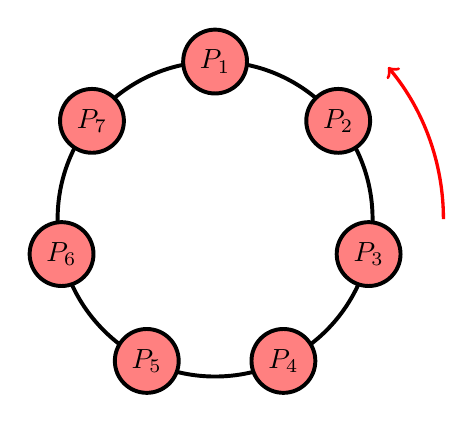
\begin{tikzpicture}
    \draw [line width=0.5mm, draw] (0:2) arc (0:360:20mm);
    \foreach \i in {1,...,7}{
        \node[line width=0.5mm, draw, circle,fill=red!50] (P_\i) at (-360/7 * \i+90+360/7:2cm) {$P_{\i}$};};
    \draw [very thick, red, draw, ->] (0:2.9) arc (0:40:30mm);
\end{tikzpicture}
\caption{Een ronde tafel met zeven genodigden}
\end{figure}

Het tweede voorbeeld gaat over het maken van een halsketting met zeven kralen ($K_1, K_2, \dots, K_7$). De kralen kunnen uit een bokaal genomen worden waarin drie verschillende kleuren zitten. De halsketting heeft echter een sluiting. En dit zorgt ervoor dat er een andere vorm van symmetrie is dan bij de ronde tafel. Als de gekleurde kralen een positie verder geschoven worden, ontstaat er immers een  ketting met andere kleuren aan beide kanten van de sluiting. Je kunt de kralen dus niet roteren. Maar je kunt deze halsketting wel lijnspiegelen zodat de sluiting op haar plaats blijft. Door deze lijnspiegeling verandert de kraal in essentie niet.

Zonder rekening te houden met de symmetrie van het spiegelen, zijn er $\overline{V}_3^7=2187$ verschillende kleuringen voor de halsketting mogelijk. Dit aantal zal drastisch inkrimpen als er spiegelingen worden toegestaan. We rekenen deze inkrimping even uit.
 
\begin{figure}[H]
\centering
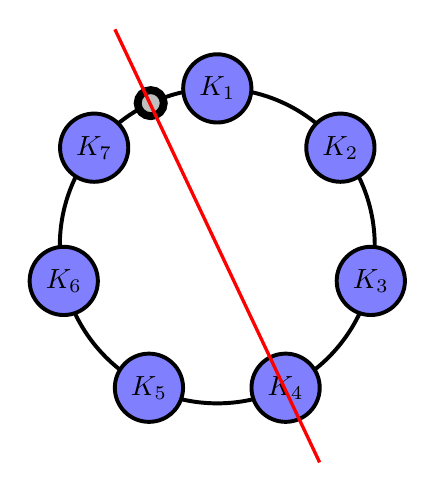
\begin{tikzpicture}
    \draw [line width=0.5mm, draw] (0:2) arc (0:360:20mm);
    \foreach \i in {1,...,7}{
        \node[line width=0.5mm, draw, circle,fill=blue!50] (P_\i) at (-360/7 * \i+90+360/7:2cm) {$K_{\i}$};};
    \node[line width=1 mm, draw, circle, fill=gray!50] (S) at (115:2cm) {};
    \draw[very thick, red] (1.3,-2.75)--(-1.3,2.75);
\end{tikzpicture}
\caption{Een halsketting met zeven kralen en een sluiting}
\label{kralen}
\end{figure}

Er zijn kleuringen die ongewijzigd blijven bij het spiegelen. Het zijn de kleuringen die symmetrisch zijn ten opzichte van de spiegelas. Op figuur \ref{kralen} zie je dat je bijvoorbeeld de kleuren van $K_1, K_2, K_3$ en $K_4$ vrij kan kiezen om een symmetrische ketting te maken. Door de keuze van $K_1, K_2, K_3$ en $K_4$ liggen ook $K_5$, $K_6$ en $K_7$ vast. In totaal zijn er $3^4=81$ kettingen die de getekende rechte als symmetrie-as hebben. 

De overige $3^7-3^4=2106$ kettingen horen twee aan twee bij elkaar. De kleuringen zijn elkaars spiegelbeeld ten opzichte van de symmetrie-as. Maar in essentie bepalen twee spiegelsymmetrische kleuringen eenzelfde halssnoer. Dit aantal halveren we dus. We vinden $\frac{3^7-3^4}{2}=1053$ verschillende halskettingen van dit type.

Door de invoering van de symmetrie, blijven er nog maar $81+1053=1134$ verschillende kettingen over. 

Om een goede reductie te doen van het aantal kleuringen als er symmetrie wordt toegevoegd, moeten we duidelijk omschrijven welke transformaties er op het te kleuren object mogen worden uitgevoerd. Bij elke transformatie moet er een studie gemaakt worden van het aantal kleuringen dat ongewijzigd blijft. Deze kleuringen noemen we de \emph{invariante kleuringen} of de \emph{invarianten} van een transformatie. 

Vraag je je ondertussen af of er ook een lijnspiegeling mag uitgevoerd worden bij het voorbeeld van de tafelschikkingen? De tafel zelf mag je zeker niet lijnspiegelen want dan staan de poten naar omhoog.

En de genodigden? Kun je die lijnspiegelen (zonder ze met de poten omhoog te zetten)? Als linkshandige zit ik meestal aan de linkerkant van mijn rechtshandige partner. Bij het oplepelen van soep blijkt dit wel eens nuttig te zijn. Als we omgekeerd naast elkaar zouden plaatsnemen, lijkt de situatie me essentieel verschillend te zijn.

\tussentitel{Theoretische achtergrond}
Isometrieën die een object op zichzelf afbeelden, noemen we \emph{symmetrieën}. Je kunt een vierkant in het vlak op zichzelf afbeelden door een rotatie, een lijnspiegeling, een puntspiegeling of door niets te doen. Ja, ook niets doen, is een vorm van transformeren. We noemen deze transformatie de \emph{identieke transformatie}. 

Ook in drie dimensies kunnen we een object op zichzelf afbeelden. Denk bijvoorbeeld aan een kubus. Symmetrieën van een kubus zijn de \emph{identieke transformatie}, een rotatie over 90°, 180° of $-$90° rond de verbindingslijn van de middens van overstaande zijvlakken, een rotatie over 180° over de verbindingslijn tussen middens van de overstaande ribben en een rotatie over 120° of $-$120° rond de verbindingslijn tussen twee overstaande hoekpunten, zie figuur \ref{rotaties}. 

Verder zijn er nog symmetrieën die de kubus binnenstebuiten keren zoals de vlak- en puntspiegelingen. Fysisch gezien kun je een kubus binnenstebuiten keren als hij van soepel rubber gemaakt is en als er ergens een gaatje in zit. Maar deze rubbertransformaties laten we buiten beschouwing. We werken met een kubus die van hout gemaakt is en we beschouwen enkel de symmetrieën die je als verplaatsingen kunt realiseren.

\begin{figure}[H]
\centering
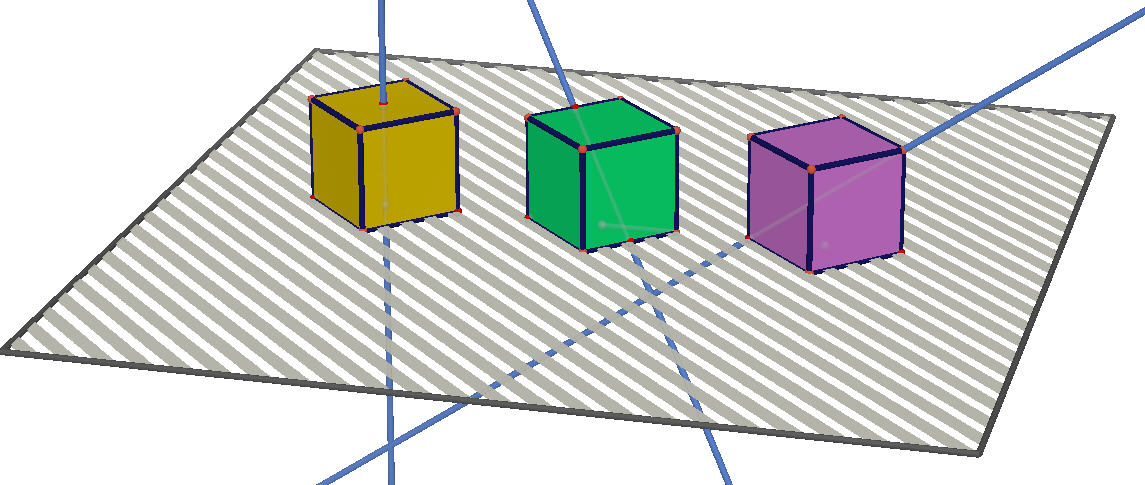
\includegraphics[width=\linewidth]{figurenAuteur/rotaties.jpg}
\caption{Rotaties die de kubus op zichzelf afbeelden}
\label{rotaties}
\end{figure}

Het tellen, inventariseren en classificeren van de symmetrieën van een vlak of van een ruimtelijk object, is een mooie stap naar abstracte wiskunde, meer bepaald naar de groepentheorie (Roelens 2004). Je kunt in deze context makkelijk zien  dat de verzameling van de symmetrieën van de houten kubus gesloten is voor de samenstelling en dat ook de verzameling van de symmetrieën van een rubberen kubus deze eigenschap heeft.

Het is ook niet moeilijk om te berekenen op hoeveel manieren een houten kubus op zichzelf kan worden afgebeeld. Je doet dit in stapjes. Je neemt een houten kubus die je in een congruent hologram wilt plaatsen. Eerst kies je welk houten hoekpunt je links-boven-voor wilt plaatsen. Er zijn 8 mogelijkheden. Dan beslis je welk hoekpunt je rechts-boven-voor wilt plaatsen. Door te draaien met de kubus rond het pas geplaatste hoekpunt komen er nog maar 3 hoekpunten in aanmerking om de houten kubus verder op zijn plaats te zetten. In totaal zijn er 24 mogelijkheden om de houten kubus in zijn hologram te plaatsen. Precies zoveel symmetrieën zijn er van een houten kubus.

Na deze bespiegelingen over symmetrieën leggen we de link met de kleuringen. Voor elk van de symmetrieën van een object kun je berekenen hoeveel kleuringen er ongewijzigd blijven. Dit aantal invariante kleuringen hangt af van de aard van de symmetrie maar ook van het aantal kleuren dat gebruikt mag worden. Het totale aantal kleuringen van het object kan nu berekend worden met de telstelling van Burnside.

De telstelling draagt de naam van de Britse wiskundige William Burnside (1852-1927), een voorloper in het onderzoek van eindige groepen. Deze stelling was lang voor de publicatie van Burnside in 1897 gekend. In 1845 bleek ze al in gebruik te zijn door Cauchy. In zijn werk \emph{On the Theory of Groups of Finite Order} citeerde hij de stelling, die hij toeschreef aan zijn wiskundige collega, Frobenius. Een interessante schets van een bewijs voor de telstelling vind je in (Bos 2017).

\begin{stellingkadertwee}
{Telstelling}{Stelling van Burnside}{Het aantal verschillende kleuringen van een symmetrisch object is gelijk aan het gemiddelde aantal invariante kleuringen per symmetrie.}
\end{stellingkadertwee}



\tussentitel{Toepassing op de stelling van Burnside}

Als je de zijvlakken van een kubus wilt verven en je beschikt slechts over twee potten verf, een zwarte en een witte, dan kun je wellicht zonder formules uitrekenen hoeveel mogelijkheden er zijn.

\begin{opsomming}
\item{Er zijn twee kubussen die monochroom gekleurd zijn: een effen witte en een effen zwarte}
\item{Twee kleuringen hebben vijf vlakken van de ene kleur en één enkele van de andere kleur. De ene kleuring is complementair aan de andere: wit wordt zwart en zwart wordt wit.}
\item{Er zijn vier kleuringen met twee vlakken in de ene kleur en vier vlakken in de andere kleur. De twee afwijkende vlakken kunnen tegenover elkaar liggen maar ze kunnen ook aangrenzend zijn. Dit kan met twee witte vlakken en vier zwarte en met de complementaire kleuren.}
\item{Tot slot zijn er twee kleuringen mogelijk met de helft van de zijvlakken wit de andere helft zwart. In het ene geval komen de witte zijvlakken in een hoekpunt samen en in het ander geval vormen de witte zijvlakken een brugje.}

\end{opsomming}

In totaal zijn er 10 kleuringen voor de zijvlakken van een houten kubus als je over twee kleuren verf beschikt en als je de zijvlakken in een zuivere kleur wilt schilderen. Voor drie verschillende kleuren verf denk ik niet dat het nog lukt om alle mogelijkheden op te sommen zonder er eentje te vergeten. Met de telstelling van Burnside kunnen we de ambities bij het tellen iets hoger leggen. Ziehier het kleurprobleem dat we samen met de lezer zullen oplossen.


\begin{stellingkadertwee}
{Kleurprobleem}{Zijvlakken van de kubus}{Stel dat je de zijvlakken van een houten kubus wilt kleuren en je beschikt hiervoor over $x$ verschillende kleuren verf. Er mogen geen kleuren gemengd worden. Elk zijvlak moet in een zuivere kleur geverfd worden. Twee kleuringen van de kubus zijn gelijk indien de ene kleuring van de kubus kan omgerold worden in de andere. Bereken onder deze beperkingen het totaal aantal verschillende kleuringen voor deze kubus.}
\end{stellingkadertwee}

We overlopen eerst alle symmetrieën van de kubus en tellen telkens hoeveel invariante kleuringen er zijn. Laten we beginnen met de identieke transformatie. Daar is er slechts $1$ van. En elke kleuring blijft zichzelf onder de identieke transformatie. De zes zijvlakken kunnen op $x^6$ manieren gekleurd worden en al deze kleuringen zijn invarianten. We onthouden voor de identieke transformatie enkel de getallen $1$ en $x^6$.

Vervolgens komen de rotaties aan de beurt rond de verbindingsrechten van de middens van overstaande zijvlakken. Er zijn rotaties van 180°. Zo zijn er in totaal 3. Het aantal invarianten voor elk van deze rotaties is $x^4$ (verklaring: voor een verticale symmetrieas heb je een aparte kleur voor het ondervlak, eentje voor het bovenvlak en een kleur voor elk paar overstaande zijvlakken). 

\begin{figure}[H]
\centering
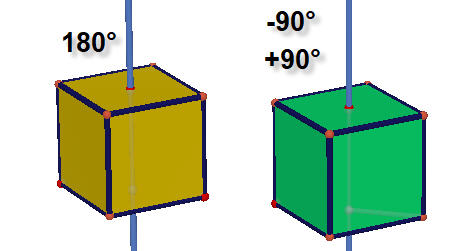
\includegraphics[width=0.9\linewidth]{figurenAuteur/geval1.jpg}
\caption{Rotaties rond verbindingsrechten van de middens van overstaande zijvlakken}
\label{eerste}
\end{figure}

Er zijn ook rotaties over een rechte hoek. Van deze soort zijn er 6. En elk van de zes rotaties heeft $x^3$ invariante kleuringen (verklaar!). We onthouden de getallen $3$ en $x^4$ en 6 en $x^3$. 

\begin{figure}[H]
\centering
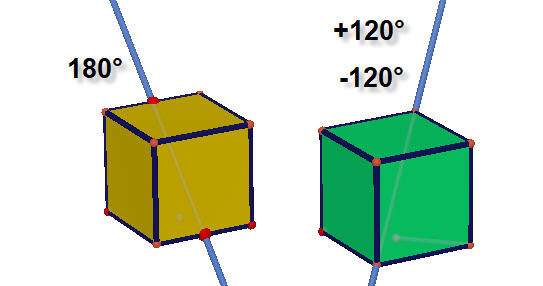
\includegraphics[width=\linewidth]{figurenAuteur/geval2.jpg}
\caption{Rotaties rond verbindingsrechten van de middens van overstaande ribben en rond verbindingsrechten van overstaande hoekpunten}
\label{tweede}
\end{figure}

Tot slot resten er nog twee soorten symmetrieën: de rotaties rond de verbindingsrechten van de middens van overstaande ribben en de rotaties rond de verbindingsrechten van overstaande hoekpunten. Van de eerste soort zijn er 6. Het aantal invariante kleuringen voor zulke halfturns is $x^3$ (ga dit na!). En van de tweede soort zijn er 8. Per omwentelingsas is er een rotatie over 120° en een rotatie over $-$120°. Je kunt berekenen dat er voor deze rotaties $x^2$ invarianten zijn.

We vatten al deze berekeningen samen in de onderstaande tabel.

Als we de aantallen in de voorlaatste kolom optellen vinden we 24 symmetrieën. Dit aantal hadden we ook eerder al gevonden. 

Het totale aantal invarianten, berekend door alle transformaties in acht te nemen, is:
\[1 \cdot x^6+3 \cdot x^4+12 \cdot x^3+8\cdot x^2.\]
Hieruit volgt dat het gemiddelde aantal invarianten per symmetrie gelijk is aan:
\[k(x)=\frac{1 \cdot x^6+3 \cdot x^4+12 \cdot x^3+8\cdot x^2}{24}.\]

De formule $k(x)$ wijst op een breuk maar voor elke natuurlijke waarde $x$ geeft $k(x)$ een geheel getal. Dit geheel getal stelt het aantal kleuringen van de houten kubus voor als je beschikt over $x$ verschillende kleuren. Het zou een onbegonnen werk geweest zijn de getallen uit de onderstaande tabel te achterhalen door manueel te tellen.

\end{multicols}
\begin{center}
    \begin{tabular}{ |p{6 cm} |c |c|c|}
    \hline
    &&&\\
    \bf{beschrijving van symmetrie} & \bf{rotatiehoek} & \bf{aantal symmetrieën} & \bf{aantal invarianten} \\ 
    &&&\\
    \hline
    &&&\\
   \emph{identieke transformatie} & & 1 & $x^6$ \\ 
   &&&\\
   \emph{rotatie} rond as die de verbinding is tussen middens van overstaande zijvlakken & 180° & 3 & $x^4$ \\ 
   &&&\\
   \emph{rotatie }rond as die de verbinding is tussen middens van overstaande zijvlakken & +90° of $-$90° & 6 & $x^3$ \\
   &&&\\
   \emph{rotatie} rond as die de verbinding is tussen middens van ribben & 180° & 6 & $x^3$ \\ 
   &&&\\
   \emph{rotatie} rond as die de verbinding is tussen overstaande hoekpunten & +120° of $-$120° & 8& $x^2$ \\
    &&&\\
    \hline
    \end{tabular}
\end{center}
\vspace{0.5cm}
\begin{multicols}{2}

\begin{center}
    \begin{tabular}{ |c | c c c c c c c|}
    \hline
    &&&&&&&\\
    $x$ & 1 & 2 & 3 & 4 & 5 & 6 & 7\\ 
    &&&&&&&\\
    \hline
    &&&&&&&\\
    $k(x)$ & 1 & 10 & 57 & 240 & 800 & 2226 & 5390\\
    &&&&&&&\\
    \hline
    \end{tabular}
\end{center}

Merken we nog even op dat de graad van de telveelterm $k(x)$ gelijk is aan het aantal onderdelen dat te kleuren is. De coëfficiënten van de veelterm hangen louter af van de symmetrieën die er in het object zitten.

\tussentitel{Origamibloemen en rietjesconstructies}

Het tellen van kleuringen is een geschikt onderwerp voor een zelfstandig onderzoek door leerlingen. Ze kunnen starten met vlakke kleuringen en eindigen met ruimtelijke. Het eenvoudigste is om zijvlakken, ribben, hoekpunten van zuivere meetkundige objecten te kleuren, zoals de zijvlakken van een kubus. Maar de leerlingen kunnen ook gebruiks- en kunstvoorwerpen met een bepaalde symmetrie in kleur zetten. Op knutselsites vind je voldoende inspiratie voor het tellen van kleuringen.

\begin{figure}[H]
\centering
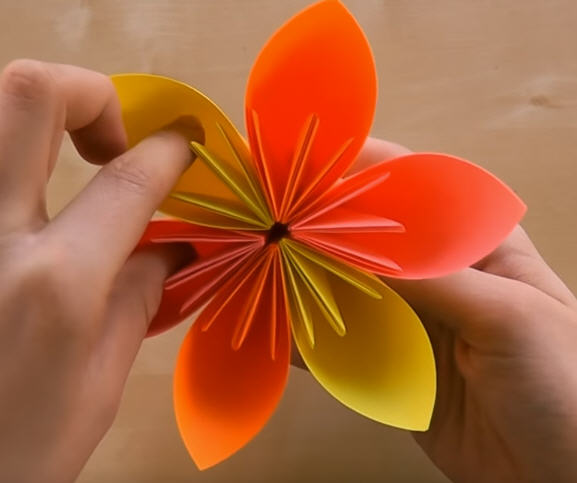
\includegraphics[width=0.8\linewidth]{figurenAuteur/bloem.jpg}
\caption{Een origamibloem met zes blaadjes}
\label{bloem}
\end{figure}

Op figuur \ref{bloem} zie je een zesbladige bloem die gemaakt is via origami of papiervouwkunst. De kelkblaadjes zijn gekleurd in geel en oranje. Net zoals bij de kubus moeten hier 6 onderdelen (hier: kelkblaadjes met drie meeldraden) gekleurd worden. Hoeveel verschillende gekleurde bloemen kan men volgens dit model maken indien men beschikt over $x$ verschillende kleuren? Hou er rekening mee dat de bloem een zesvoudige rotatiesymmetrie heeft. De voor- en de achterkant van de bloem zien er verschillend uit.

Als je over twee kleuren beschikt, zoals op de figuur, is het aantal verschillende origamibloemen nog uit het hoofd te tellen. Je vindt er 14. Maar als het aantal kleuren hoger wordt, moet je een studie maken van de verschillende symmetrieën van de bloem. Dit zijn er slechts 6. De aantallen invariante kleuringen bij elke symmetrie zijn eenvoudig te berekenen. Wil je deze vraag iets moeilijker maken dan vervang je de 6 kelkblaadjes door bijvoorbeeld 15 kelkblaadjes.

Op figuur \ref{tetraeder} zie je een tetraëder die gemaakt is van 6 rietjes. Ze zijn gekleurd in rood, geel en blauw. Net zoals bij de kubus en bij de origamibloem moeten ook hier 6 onderdelen een kleur krijgen. Hoeveel verschillende kleuringen van de ribben van de tetraëder bestaan er als je beschikt over $x$ kleuren? Je mag met de tetraëder rollen maar je mag hem niet binnenstebuiten halen m.a.w. je mag een top van de piramide niet door de basis trekken (of de top door het grondvlak spiegelen).

Bij deze oefening is het iets moeilijker om alle kleuringen te tellen want er zijn iets meer symmetrieën dan bij het voorgaande probleem. Er zijn twee soorten rotatie-assen in deze figuur aanwezig. In totaal zijn er 12 symmetrieën.  Als je de tetraëder ook binnenstebuiten zou kunnen trekken, beschikken we over 24 symmetrieën. Hierdoor zou de vraag heel wat moeilijker worden.  

\begin{figure}[H]
\centering
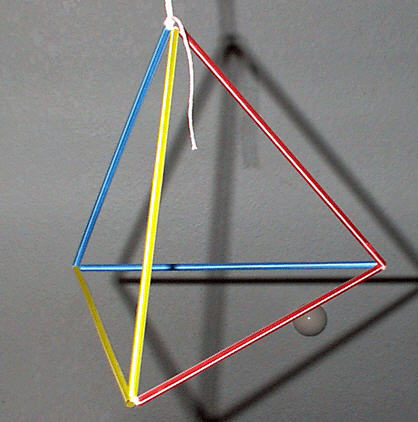
\includegraphics[width=0.8\linewidth]{figurenAuteur/tetraeder.jpg}
\caption{Een tetraëder met zes rietjes}
\label{tetraeder}
\end{figure}

Als je slechts twee kleuren zou gebruiken, kun je de 12 mogelijke kleuringen van de tetraeder makkelijk omschrijven. Je hebt voor de telling geen formules nodig. Dit resultaat kun je gebruiken om de algemene formule voor het aantal kleuringen van de tetraëder met $x$ kleuren te controleren.

\section {Een telprobleem waar muziek in zit}


Al jaren vraag ik me af hoeveel akkoorden met drie verschillende noten er bestaan en hoeveel met vier noten? Het lijken me er ontzaglijk veel. Maar ik besefte pas dat ik het mis had toen ik (Bos, 2017) las. De berekening van deze aantallen akkoorden zijn in het Zebra-boekje opgenomen als een vrije eindopdracht voor de leerlingen. De laatste paragraaf van deze loep is bedoeld voor de muziekminnende en artistieke leerkracht en leerling. Muziek en wiskunde zijn interesses die elkaar wel eens raken.


\tussentitel {Drieklanken}

Een drieklank is een opeenstapeling van drie verschillende tonen. Om visueel te laten zien dat de drie noten tegelijkertijd moeten gespeeld of gezongen worden, noteren we ze boven elkaar op een notenbalk. In figuur \ref{grootklein} zie je de grote drieklank (of het grote terstsakkoord) do-mi-sol en de kleine drieklank (of het kleine tertsakkoord) do-mi$b$-sol. Elk akkoord heeft een eigen karakter. Het grote tertsakkoord klinkt vrolijk, het kleine klinkt droef. Als je de drie noten van een drieklank parallel verschuift over de notenbalk dan blijft het karakter behouden. Vrolijk blijft vrolijk. Droevig blijft droevig.

\begin{figure}[H]
\centering
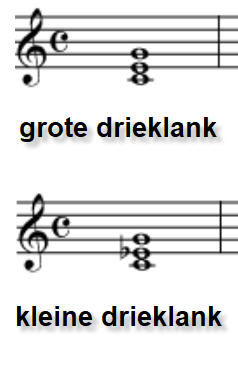
\includegraphics[width=0.4\linewidth]{figurenAuteur/grootenklein.jpg}
\caption{Twee drieklanken met een verschillende sfeer}
\label{grootklein}
\end{figure}

De grote en kleine drieklank klinken welluidend. De drie noten liggen immers niet vlak naast elkaar. Deze klassieke akkoorden stralen rust uit. Het akkoord re-mi-sol klinkt een beetje dissonanter omdat de re en mi tegen elkaar aan schuren. En het akkoord re-mi-fa klinkt heel wrang. De drie geclusterde noten genereren een geluidseffect dat goed zou passen bij een griezelfilm. 

De onderlinge tussenafstanden van de noten van een drieklank bepalen de sfeer ervan. De oorspronkelijke vraag kan nu muzikaler vertaald worden. Hoeveel muzikale sferen kan men oproepen door drie noten samen te laten klinken? We tellen het zo meteen uit. Eerst iets over het wiskundige model achter de drieklanken.

\tussentitel{De halvetonencirkel}

Als je een klavier van een piano of een orgel bekijkt, merk je dat de structuur zich elke twaalf halve tonen herhaalt. De afstand van 12 halve tonen noemen we een octaaf. De namen van de noten herhalen zich ook na elke cyclus van 12 halve tonen. Daarom kunnen we deze namen in een cirkel noteren, zoals in figuur \ref{notencirkel}. 

\begin{figure}[H]
\centering
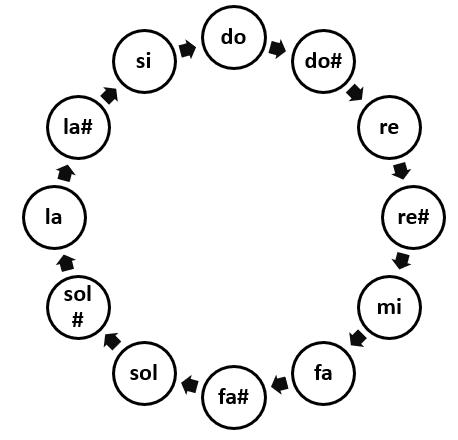
\includegraphics[width=0.8\linewidth]{figurenAuteur/halvetonencirkel.jpg}
\caption{Het octaaf, een cyclus van 12 halve tonen}
\label{notencirkel}
\end{figure}

De toonhoogte stijgt in de richting van de pijlen. In het eenvoudigste geval beginnen we een toonladder bij de do en klimmen we op tot de si. Zo hebben we een heel octaaf doorlopen. Maar we kunnen ook op een andere plaats beginnen om het octaaf te doorlopen. We zullen nu verder redeneren op het model van de halvetonencirkel en niet meer op het pianoklavier.

Bij de benamingen van de noten zijn hier kruisen genoteerd voor een verhoging met een halve toon.  Maar we hadden net zo goed de notatie met de mollen kunnen gebruiken voor een verlaging met een halve toon. Onthoud wel: re$\#$ (re kruis) is gelijk aan mi$b$ (mi mol) en fa$\#$ (fa kruis) is gelijk aan sol$b$ (sol mol).

\tussentitel{Drieklanken in de halvetonencirkel}

Een drieklank kun je aanduiden in de halvetonencirkel door precies 3 van de 12 cirkeltjes in te kleuren. In de figuren \ref{mineur} en \ref{majeur} zie je de afbeelding van het kleine tertsakkoord do-mi$b$-sol en die van het grote tertsakkoord do-mi-sol.

Ook al zouden er geen notennamen in de cirkeltjes staan, visueel zijn deze akkoorden makkelijk uit de posities van de gekleurde cirkeltjes op te maken. Het verschil zit in de tussenafstanden tussen de cirkeltjes die tot het akkoord behoren.

Om cyclisch van de ene noot van het akkoord naar de volgende te hoppen, zijn er drie afstanden met pijlen te overbruggen. Kijk alleen naar de twee kleinste afstanden. De derde tussenafstand ligt immers vast wanneer de twee kleinste afstanden vast liggen. Bij het kleine tertsakkoord moeten er eerst 3 pijlen genomen worden (van do naar mi$b$) en daarna 4 (van mi$b$ naar sol). Bij het grote tertsakkoord moeten er eerst 4 pijlen genomen worden (van do naar mi) en daarna 3 (van mi naar sol). Het temperament van een akkoord wordt zo gekarakteriseerd in twee kengetallen.

\begin{figure}[H]
\centering
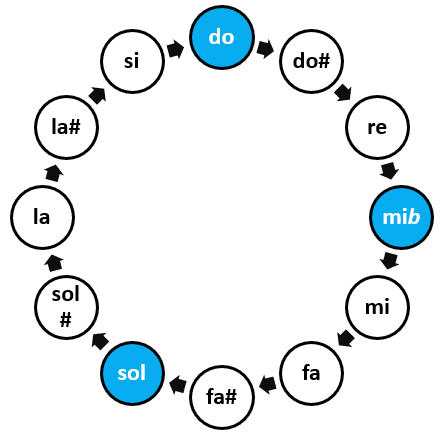
\includegraphics[width=0.8\linewidth]{figurenAuteur/domibsol.jpg}
\caption{Het kleine tertsakkoord do-mi$b$-sol}
\label{mineur}
\end{figure}

\begin{figure}[H]
\centering
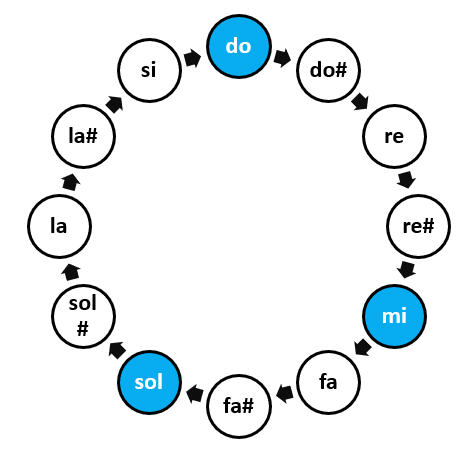
\includegraphics[width=0.8\linewidth]{figurenAuteur/domisol.jpg}
\caption{Het grote tertsakkoord do-mi-sol}
\label{majeur}
\end{figure}


\tussentitel{Roteren en spiegelen van een akkoord}

We stellen ons nu de vraag of een akkoord verandert door de gekleurde cirkeltjes in de halvetonencirkel te roteren of te spiegelen. Kijken we eerst naar de rotatie. 

Als we het grote tertsakkoord do-mi-sol over een twaalfde van een volledige omwenteling  roteren naar het akkoord do$\#$-fa-sol$\#$, klinkt het een halve toon hoger. Aan de sfeer is er niets veranderd. We kunnen dit akkoord beschouwen als een oude bekende en rekenen het niet mee in de telling van de verschillende drieklanken. De kengetallen van het akkoord blijven immers gelijk aan 4 en 3.

\begin{figure}[H]
\centering
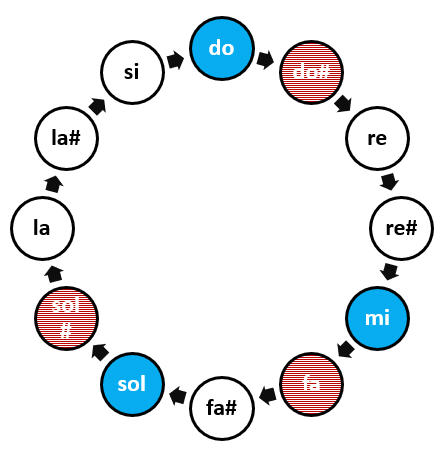
\includegraphics[width=0.8\linewidth]{figurenAuteur/dokfasolk.jpg}
\caption{Het grote tertsakkoord geroteerd}
\label{majeurgespiegeld}
\end{figure}

\begin{figure}[H]
\centering
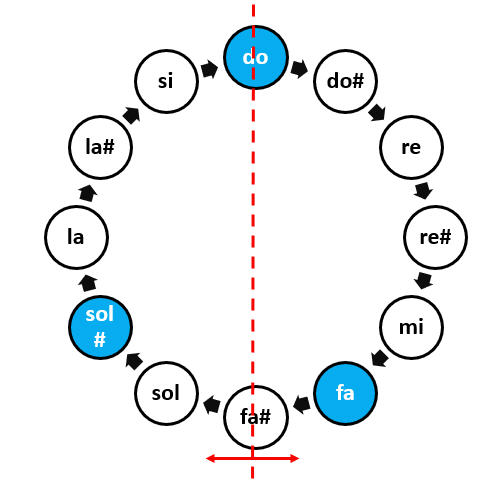
\includegraphics[width=0.8\linewidth]{figurenAuteur/dofasolk.jpg}
\caption{Het grote tertsakkoord gespiegeld}
\label{majeurgeroteerd}
\end{figure}

De spiegelingen zijn iets moeilijker. Stel dat we de gekleurde cirkeltjes van het grote tertsakkoord do-mi-sol spiegelen rond de verticale door het middelpunt van de halvetonencirkel. Dan komen we uit bij het akkoord do-fa-sol$\#$. Dit akkoord is wel degelijk verschillend van het grote tertsakkoord. De karakteristieke getallen zijn 3 en 4. De gespiegelde van het grote tertsakkoord klinkt als het kleine tertsakkoord. 

Door te spiegelen rond een as krijgen we meestal een ander akkoord (een akkoord met andere kengetallen, een akkoord dat een andere sfeer oproept). Door te roteren blijft een akkoord altijd hetzelfde klinken (de kengetallen veranderen niet, de sfeer ook niet).

\tussentitel{En nu de telling}

Als je van de 12 cirkeltjes in de halvetonencirkel er precies 3 mag inkleuren, dan kunnen we het aantal inkleuringen berekenen met een combinatie: $C_{12}^3=220$. Deze inkleuringen zou je in groepjes per 12 moeten samennemen. Je krijgt telkens 12 akkoorden met dezelfde kengetallen maar met een andere positie op de halvetonencirkel. Groeperen per 12 lukt echter niet helemaal omdat het getal 220 is niet deelbaar door 12.

Sommige akkoorden kun je niet met 12 samennemen. Denk maar aan het akkoord do-mi-sol$\#$, dat zijn bolletjes heeft op de hoekpunten van een gelijkzijdige driehoek. 


\begin{figure}[H]
\centering
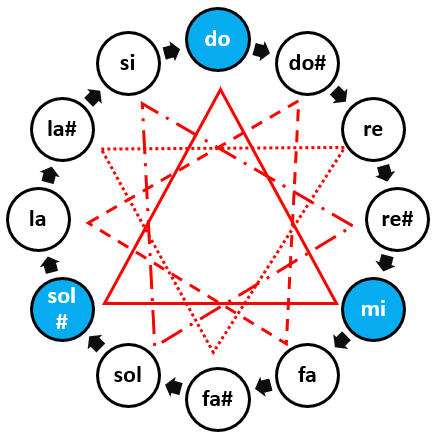
\includegraphics[width=0.8\linewidth]{figurenAuteur/domisolk.jpg}
\caption{Vier vergrote drieklanken}
\label{vergroot}
\end{figure}

We noemen dit merkwaardige akkoord een vergrote drieklank. De kengetallen zijn 4 en 4. In de halvetonencirkel van figuur \ref{vergroot} zie je vier vergrote drieklanken die aangegeven zijn door gelijkzijdige driehoeken van een verschillend lijntype. Deze vier akkoorden stralen dezelfde klanksfeer uit. 

Een vergrote drieklank heeft de eigenschap  invariant te zijn onder een rotatie over 120° en onder een rotatie over 240°. Alle andere drieklanken zijn enkel invariant onder de identieke transformatie. Deze opmerking geeft een aanwijzing in de richting van het lemma van Burnside. Maar ook zonder op dit lemma te steunen, vinden we het antwoord op de vraag.

Van de 220 oorspronkelijke kleuringen worden er 4 samengenomen tot 1. Dat zijn de vier vergrote drieklanken. De overige 216 worden in groepjes van 12 samengenomen. Dat zijn 18 groepjes die bestemd zijn voor akkoorden zonder rotatiesymmetrie. We vinden dus 19 verschillende akkoorden. 

Nu de berekening is gemaakt, is het nog een heel gedoe om al deze akkoorden op te sommen. We zetten ze hieronder netjes in een tabel. Links zie je de meest geclusterde drieklanken. Rechts de drieklanken met een wijdere spreiding. Uiterst rechts vind je de merkwaardigste drieklank: de vergrote drieklank. 

Wil je alle mogelijke drieklanken na elkaar horen, zet je dan maar achter de piano en speel de partituur uit figuur \ref{negentien} ... of dan ga je naar de website van UW en klik je het bijbehorende audiobestand aan.

Als je nog zin hebt om de hele redenering over te doen voor de berekening van het aantal vierklanken: het zijn er 43. Let op: er zijn symmetrische vierklanken die met drie moeten gebundeld worden (de bolletjes in de halvetonencirkel liggen op de hoekpunten van een vierkant), er zijn symmetrische vierklanken die je met zes moet samennemen (de bolletjes liggen op de hoekpunten van een rechthoek) en er zijn asymmetrische vierklanken die je met twaalf moet samennemen ...

\end{multicols}

\begin{center}
    \footnotesize
    \begin{tabular}{|ccccccccccccccccccc|}
    \hline
    &&&&&&&&&&&&&&&&&&\\
   1 & 2 & 3 & 4 & 5 & 6 & 7 & 8 & 9 & 10 & 11 & 12 &  13 & 14 & 15 & 16 & 17 & 18 & 19 \\ 
   &&&&&&&&&&&&&&&&&&\\
    \hline
    &&&&&&&&&&&&&&&&&&\\
    do & do & do & do & do & do & do & do & do & do & do & do &  do & do & do & do & do & do & do \\ 
    do$\#$ & do$\#$ & re & do$\#$ & re & re$\#$ & do$\#$ & re & re$\#$ & mi & do$\#$ & re &  re$\#$ & mi & fa & re & re$\#$ & mi & mi \\ 
    re & re$\#$ & re$\#$ & mi & mi & mi & fa & fa & fa & fa & fa$\#$ & fa$\#$ &  fa$\#$ & fa$\#$ & fa$\#$ & sol & sol & sol & sol$\#$ \\ 
    &&&&&&&&&&&&&&&&&&\\
    \hline
    \end{tabular}
\end{center}

\begin{figure}[H]
\centering
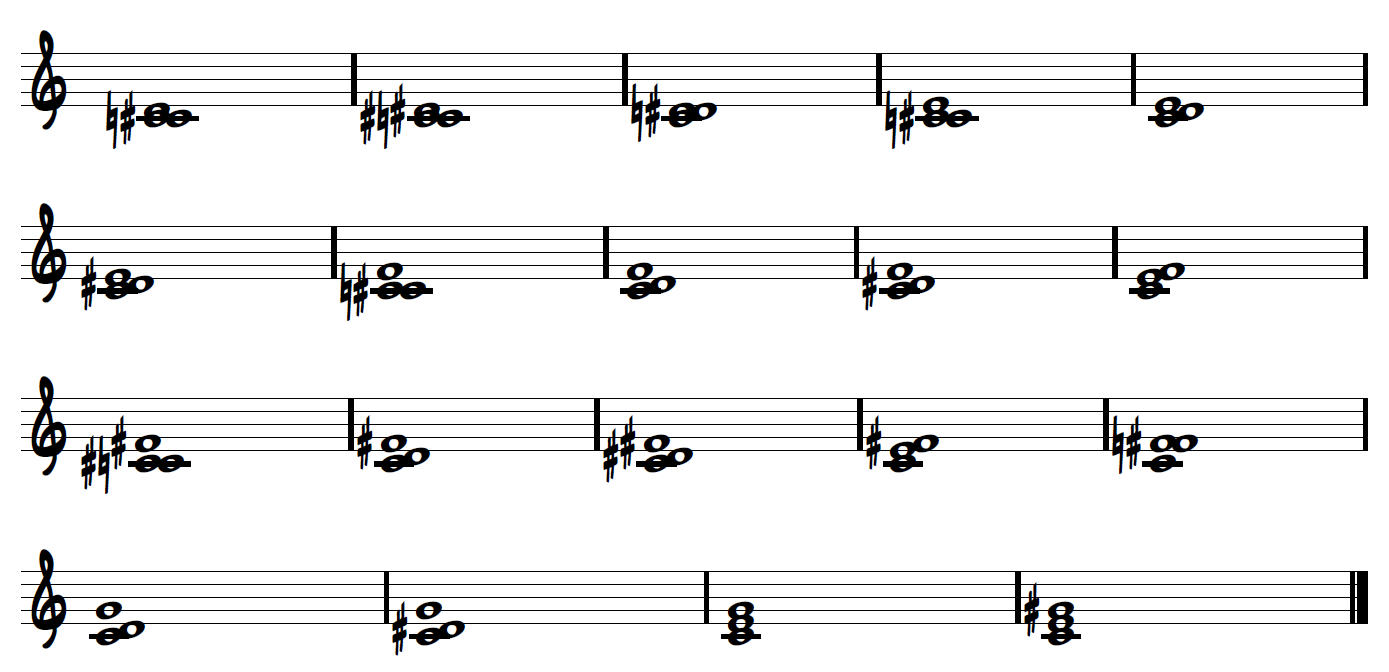
\includegraphics[width=\linewidth]{figurenAuteur/alledrieklanken.jpg}
\caption{Negentien verschillende drieklanken}
\label{negentien}
\end{figure}


\begin{multicols}{2}

\end{multicols}



\stopcontents[mainsections]			        % altijd laten staan, opsomming in inhoudstafel enkel tot loep beperken
 

% bronnen toevoegen
\begin{bronnen}
\item Bos, R., Tak, S. (2017).\emph{ Symmetrie in telproblemen en puzzels}. Amsterdam: Epsilon Uitgaven. ISBN 978-90-5041-116-0

\item Discrete wiskunde (vwo a). \emph{Tellen}. Geraadpleegd op 04/03/2013,  www.math4all.nl/overzichten/vwo-a/20

\item Eggermont, H., Roelens, M. (1989). Combinatieleer. \emph{Uitwiskeling 5/3}, 25-49.

\item Gevers, P. et al (2004). \emph{Kansrekenen}. Delta 5/6 (3/4 lesuren). Wolters Plantyn.

\item Roelens, M. (2004). Symmetrische figuren. \emph{Uitwiskeling 20/2}, 19-23.




\end{bronnen}

